\documentclass[conference]{IEEEtran}
\IEEEoverridecommandlockouts
% The preceding line is only needed to identify funding in the first footnote. If that is unneeded, please comment it out.
\usepackage{cite}
\usepackage{amsmath,amssymb,amsfonts}
\usepackage{algorithmic}
\usepackage{graphicx}
\usepackage{textcomp}
\usepackage{xcolor}
\usepackage{orcidlink}
\usepackage{graphicx}
\usepackage{hyperref}
\usepackage{multicol}
\usepackage[final]{changes}
\usepackage{url}
\usepackage{amsmath}
\usepackage{bm}
\usepackage{multirow}
\usepackage{tcolorbox}
\usepackage{rotating}
\usepackage{latexsym,amssymb,amsmath}
\usepackage{makecell}
\usepackage{xspace}
\usepackage{paralist}
\usepackage{wrapfig}
\usepackage{adjustbox}
\usepackage{cite}
\usepackage{todonotes}
\usepackage{graphicx}
\usepackage{xcolor,color}
\usepackage{subfig}
\usepackage{tikz}
\usepackage{calc}

\usepackage{tabularx}
\usepackage{booktabs}

\usepackage{ulem}

%\usepackage{kbordermatrix}
\usepackage{amsmath,amsfonts}
\usepackage{braket}
\usepackage{xfrac}

\usepackage{pifont}
\usepackage{amssymb}
\usepackage{paralist}
\usepackage[inline]{enumitem}

\newcommand{\pmin}{\rho}

\newcommand{\const}[1]{\mathsf{#1}}

\newcommand{\alphabet}{\Sigma}
\newcommand{\tasks}{\mathcal{A}}
\newcommand{\hidden}{\tau}

\newcommand{\uswn}{SWN\xspace}
\newcommand{\net}{\ensuremath{N}}
\newcommand{\tg}{\ensuremath{G}}
\newcommand{\closed}[1]{\overline{#1}}
\newcommand{\marking}{m}
\newcommand{\enaset}[2]{E_{#2}(#1)}
\newcommand{\fire}[4]{#1\xrightarrow{#2}_{#4}#3}
\newcommand{\probt}[3]{\mathbb{P}_{#2,#3}(#1)}
\newcommand{\prob}[2]{\mathbb{P}_{#2}(#1)}
\newcommand{\rg}[1]{RG(#1)}
\newcommand{\ind}[1]{\textnormal{\texttt{#1}}}
\newcommand{\seq}{\eta}
\newcommand{\run}{\xi}
\newcommand{\trace}{\sigma'}
\newcommand{\traces}[1]{\mathit{traces}(#1)}
\newcommand{\ptraces}[2]{\mathit{ptraces}_{#2}(#1)}

\newcommand{\nreach}[3][]{#2 \overset{#1}{\rightsquigarrow} #3}
\newcommand{\runs}[2]{runs_{#2}(#1)}
\newcommand{\seqs}[2]{seqs_{#2}(#1)}
\newcommand{\transp}[1]{#1^\top}
\newcommand{\embed}{\phi}
\newcommand{\trembed}{{\embed^{\text{tr}}}}
\newcommand{\gorgembed}{{\embed^{g}}}


\newcommand{\pa}{\rho_{23}}
\newcommand{\pb}{\rho_{24}}
\newcommand{\pc}{\rho_{55}}
\newcommand{\pd}{\rho_{65}}
\newcommand{\pe}{\rho_{67}}
\newcommand{\pf}{\rho_{57}}

\newcommand{\logtrace}{\trace}
\newcommand{\nonlogtrace}{{\sigma}}


\newcommand{\approptoinn}[2]{\mathrel{\vcenter{
			\offinterlineskip\halign{\hfil$##$\cr
				#1\propto\cr\noalign{\kern2pt}#1\sim\cr\noalign{\kern-2pt}}}}}
\newcommand{\appropto}{\mathpalette\approptoinn\relax}


\newcommand{\unravelled}{unfolded}
\newcommand{\unravelling}{unfolding}
\newcommand{\unravel}{unfold}
\newcommand{\Ind}[1]{\ind{i}_{#1}}


%
%\def\WWITHN{def}
%\ifdefined\WWITHN
%\newcommand{\WCal}[2]{{\mathcal{W}_{#1}^{#2}}}
%\newcommand{\TBf}[2]{{\mathbf{T}_{#1}^{#2}}}
%\else
\newcommand{\TBf}[2]{{\mathbf{G}_{#1}}}
%\fi
\newcommand{\expN}{\closed{\tg_{\rg{\net}}}}

\def\EqualityHolds{itholds}
\ifdefined\EqualityHolds
\newcommand{\probarg}{\tg}
\newcommand{\WCal}[2]{\ptraces{\tg}{#1}}
\else
\newcommand{\probarg}{\expN}
\newcommand{\WCal}[2]{\ptraces{\closed{\tg_{\rg{\net}}}}{#1}}
\fi
\newcommand{\probskip}[1]{\prob{#1}{\probarg}}
\newcommand{\goldenrank}{\mathcal{R}}

\newlist{myalist}{enumerate*}{1}
\setlist[myalist]{label=\textbf{(\arabic*)}}
\newlist{mylist}{enumerate*}{1}
\setlist[mylist]{label=\textit{(\roman*)}}
\newlist{alphalist}{enumerate*}{1}
\setlist[alphalist]{label=\textbf{(\alph*)}}
\renewcommand*{\UrlFont}{\ttfamily\smaller\relax}
%%%%%%%%%%%%%%%%%%%%%%%%%%%%%%%%%%%%%%%%%%%%%%%%%%%%%%%%%%%%%%%%%%%%%%%%%%%%%%
%%% Time-stamp: "2018-09-07 18:35:03 calvanese"
%%%%%%%%%%%%%%%%%%%%%%%%%%%%%%%%%%%%%%%%%%%%%%%%%%%%%%%%%%%%%%%%%%%%%%%%%%%%%%

%%%%%%%%%%%%%%%%%%%%%%%%%% General Math

\newcommand{\A}{\ensuremath{\mathcal{A}}}
\newcommand{\B}{\ensuremath{\mathcal{B}}}
%\newcommand{\C}{\ensuremath{\mathcal{C}}}
\newcommand{\D}{\ensuremath{\mathcal{D}}}
\newcommand{\E}{\ensuremath{\mathcal{E}}}
\newcommand{\F}{\ensuremath{\mathcal{F}}}
%\newcommand{\G}{\ensuremath{\mathcal{G}}}
\renewcommand{\H}{\ensuremath{\mathcal{H}}}
\newcommand{\I}{\ensuremath{\mathcal{I}}}
\newcommand{\J}{\ensuremath{\mathcal{J}}}
\newcommand{\K}{\ensuremath{\mathcal{K}}}
\renewcommand{\L}{\ensuremath{\mathcal{L}}}
\newcommand{\M}{\ensuremath{\mathcal{M}}}
\newcommand{\N}{\ensuremath{\mathcal{N}}}
\renewcommand{\O}{\ensuremath{\mathcal{O}}}
\renewcommand{\P}{\ensuremath{\mathcal{P}}}
\newcommand{\Q}{\ensuremath{\mathcal{Q}}}
\newcommand{\R}{\ensuremath{\mathcal{R}}}
%\renewcommand{\S}{\ensuremath{\mathcal{S}}}
\newcommand{\T}{\ensuremath{\mathcal{T}}}
%\newcommand{\U}{\ensuremath{\mathcal{U}}}
\newcommand{\V}{\ensuremath{\mathcal{V}}}
\newcommand{\W}{\ensuremath{\mathcal{W}}}
\newcommand{\X}{\ensuremath{\mathcal{X}}}
\newcommand{\Y}{\ensuremath{\mathcal{Y}}}
\newcommand{\Z}{\ensuremath{\mathcal{Z}}}

%%%%%%%%%%%%%%%%%%%%%%%%%% Abbreviations

%%\newcommand{\eset}{\emptyset}
%%\newcommand{\col}{\colon}
\newcommand{\ol}[1]{\overline{#1}}                % overline
%\newcommand{\ul}[1]{\underline{#1}}               % underline
%%\newcommand{\uls}[1]{\underline{\raisebox{0pt}[0pt][0.45ex]{}#1}}
%% ul with space between text and line

\newcommand{\ra}{\rightarrow}
\newcommand{\Ra}{\Rightarrow}
\newcommand{\la}{\leftarrow}
\newcommand{\La}{\Leftarrow}
%\newcommand{\lra}{\leftrightarrow}
\newcommand{\Lra}{\Leftrightarrow}
\newcommand{\lora}{\longrightarrow}
\newcommand{\Lora}{\Longrightarrow}
\newcommand{\lola}{\longleftarrow}
\newcommand{\Lola}{\Longleftarrow}
\newcommand{\lolra}{\longleftrightarrow}
\newcommand{\Lolra}{\Longleftrightarrow}
%\newcommand{\ua}{\uparrow}
\newcommand{\Ua}{\Uparrow}
\newcommand{\da}{\downarrow}
\newcommand{\Da}{\Downarrow}
\newcommand{\uda}{\updownarrow}
\newcommand{\Uda}{\Updownarrow}

%%%%%%%%%%%%%%%%%%%%%%%%%% Relations

%%\newcommand{\incl}{\subseteq}
%%\newcommand{\imp}{\rightarrow}
\newcommand{\per}{\mbox{\bf .}}                  % period

%%%%%%%%%%%%%%%%%%%%%%%%%% Delimiters

%%\newcommand{\quotes}[1]{{\lq\lq #1\rq\rq}}
%\newcommand{\set}[1]{\{#1\}}                      % set
%\newcommand{\Set}[1]{\left\{#1\right\}}
\newcommand{\bigset}[1]{\Bigl\{#1\Bigr\}}
\newcommand{\bigmid}{\Big|}
\newcommand{\size}[1]{|{#1}|}                     % cardinality of a set
%%\newcommand{\Card}[1]{\left| #1\right|}
\newcommand{\card}[1]{\sharp #1}
\newcommand{\tup}[1]{\langle #1\rangle}            % tuple
\newcommand{\Tup}[1]{\Braket{#1}}
\newcommand{\norm}[2]{\|#1\|_{#2}}
\newcommand{\setone}[2][1]{\set{#1\cld #2}}

%%%%%%%%%%%%%%%%%%%%%%%%%% STYLING AND SPACING

%\newcommand{\inlinetitle}[1]{\smallskip\noindent\textbf{#1.}\xspace}





\newcolumntype{C}{>{\centering\arraybackslash}X}

%\makeatletter
%\g@addto@macro\normalsize{%
%\setlength{\abovecaptionskip}{-2pt}
%\setlength{\belowcaptionskip}{12pt}
%\setlength\abovedisplayskip{3pt}
%\setlength\belowdisplayskip{3pt}
%\setlength\abovedisplayshortskip{3pt}
%\setlength\belowdisplayshortskip{3pt}
%}
%\makeatother

\newcounter{dummy} 
\newcounter{dummy1} 
\newcounter{dummy2}
\newcounter{dummy3} 
\newcounter{dummy4}
\newcounter{dummy5} 
\newcounter{dummy6}
\newcounter{dummy7}
%\numberwithin{dummy}{section}

\usepackage[thmmarks,amsmath]{ntheorem}
%\theorempreskip{1pt}
%\theorempostskip{1pt}

%\theoremstyle{plain}
%\theorembodyfont{\normalfont}
%\theoremseparator{.}
%\let\definition\relax
%\theoremsymbol{\ensuremath{\square}}
%\newtheorem{definition}{Definition}


\let\proposition\relax
\let\theorem\relax
\let\lemma\relax
\let\definition\relax
\theoremseparator{.}
\theorembodyfont{\itshape}
\theoremsymbol{$\triangleleft$}
\newtheorem{theorem}[dummy]{Theorem}
\newtheorem{lemma}[dummy1]{Lemma}
\newtheorem{definition}[dummy2]{Definition}
\newtheorem{proposition}[dummy3]{Proposition}

\let\remark\relax
\let\example\relax
%\let\example*\relax
\theorembodyfont{\normalfont}
\newtheorem{example}[dummy4]{Example}
\newtheorem{remark}[dummy5]{Remark}
%\newtheorem{example*}[dummy4]{Example}


\theoremstyle{nonumberplain}
\theoremheaderfont{\itshape}
\theorembodyfont{\normalfont}
\let\proof\relax
\theoremseparator{.}
\theoremsymbol{\ensuremath{\dashv}}
\newtheorem{proof}[dummy6]{Proof}


\qedsymbol{\ensuremath{\dashv}}


%%% Local Variables:
%%% mode: latex
%%% TeX-master: "main"
%%% save-place: t
%%% End:

\usepackage{etoolbox}
\usepackage{hyperref}
\def\BibTeX{{\rm B\kern-.05em{\sc i\kern-.025em b}\kern-.08em
    T\kern-.1667em\lower.7ex\hbox{E}\kern-.125emX}}
\begin{document}

\title{Probabilistic Trace Alignments\\ as a kNN Problem\\
\thanks{This research has been partially supported by the project IDEE (FESR1133) funded by the Eur.\ Reg.\ Development Fund (ERDF) Investment for Growth and Jobs Programme 2014-2020. }
}



\author{\IEEEauthorblockN{1\textsuperscript{st} Giacomo Bergami\orcidlink{0000-0002-1844-0851}}
\IEEEauthorblockA{\textit{Dept. of Computer Science} \\
\textit{Free University of Bozen-Bolzano}\\
Bozen-Bolzano, Italy \\
gibergami@unibz.it}
\and
\IEEEauthorblockN{2\textsuperscript{nd} Fabrizio Maria Maggi\orcidlink{0000-0002-9089-6896}}
\IEEEauthorblockA{\textit{Dept. of Computer Science} \\
\textit{Free University of Bozen-Bolzano}\\
Bozen-Bolzano, Italy \\
maggi@inf.unibz.it}
\and
\IEEEauthorblockN{3\textsuperscript{rd} Marco Montali\orcidlink{0000-0002-8021-3430}}
\IEEEauthorblockA{\textit{Dept. of Computer Science} \\
\textit{Free University of Bozen-Bolzano}\\
Bozen-Bolzano, Italy \\
montali@inf.unibz.it}
\and
\IEEEauthorblockN{4\textsuperscript{th} Rafael Peñaloza\orcidlink{0000-0002-2693-5790}}
\IEEEauthorblockA{\textit{--} \\
\textit{University of Milano-Bicocca}\\
Milan, Italy \\
rafael.penaloza@unimib.it}
}


\author{
	\IEEEauthorblockN{
		Giacomo Bergami\orcidlink{0000-0002-1844-0851}\IEEEauthorrefmark{1},
		Fabrizio Maria Maggi\orcidlink{0000-0002-9089-6896}\IEEEauthorrefmark{1},
		Marco Montali\orcidlink{0000-0002-8021-3430}\IEEEauthorrefmark{1},
		Rafael Peñaloza\orcidlink{0000-0002-2693-5790}\IEEEauthorrefmark{2}}

	\IEEEauthorblockA{\IEEEauthorrefmark{1}Free University of Bozen-Bolzano, Bozen, Italy\\
		Email: gibergami@unibz.it, \{maggi,montali\}@inf.unibz.it}
	\IEEEauthorblockA{\IEEEauthorrefmark{2}University of Milano-Bicocca, Milan, Italy\\
		Email: rafael.penaloza@unimib.it}
}


\maketitle

\begin{abstract}
Alignments provide sophisticated diagnostics that pinpoint deviations in a trace with respect to a process model and their severity. However, approaches based on trace alignments use crisp process models as reference and recent probabilistic conformance checking approaches check the degree of conformance of an event log with respect to a stochastic process model instead of finding trace alignments. In this paper, for the first time, we provide a conformance checking approach based on trace alignments using stochastic Workflow nets. Conceptually, this requires to handle the two possibly contrasting forces of the cost of the alignment on the one hand and the likelihood of the model trace with respect to which the alignment is computed on the other.
\end{abstract}

\begin{IEEEkeywords}
Stochastic Petri nets, Conformance Checking, Alignments.
\end{IEEEkeywords}

\section{Introduction}


\label{introduction}
%Trace alignment is a well-known technique in conformance checking \cite{DBLP:conf/edoc/AdriansyahDA11} providing both a numerical assessment of the degree of conformance of a log trace with respect to a model, as well as a repair strategy if such trace does not conform to the given model. At the time of the writing,
%
In the existing literature on conformance checking, a common approach is based on trace alignment \cite{DBLP:conf/edoc/AdriansyahDA11}. This approach uses crisp process models as reference models. Yet, recently developed probabilistic conformance checking approaches provide a numerical quantification of the degree of conformance
%the existing approaches are used to check the degree of conformance
of an event log with a stochastic process model by either assessing the distribution discrepancies \cite{DBLP:conf/bpm/LeemansSA19}, or by exploiting entropy-based measures \cite{DBLP:conf/icpm/PolyvyanyyK19,DBLP:journals/tosem/PolyvyanyySWCM20}.
As these strategies are not based on trace alignments, these cannot be directly used to repair a given trace with one of the traces generated by a stochastic process model.
%As traces generated by such models are associated to a probability exhibiting its representativeness and relevance within the model, probabilistic trace alignment techniques should take into account the combined provision of trace probability and alignment cost.
%instead of finding trace alignments.
%
In this paper, we provide for the first time an approach for the probabilistic alignment of a trace and a stochastic reference
model. This approach is not comparable with the existing literature on probabilistic conformance checking as its output is not numeric but consists of a ranked list of alignments.
Providing different alignment options is useful since, conceptually, probabilistic trace alignment requires the analyst to 
%handle the two possibly contrasting forces of the cost of the alignment on the one hand and the likelihood of the model trace with respect to which the alignment is computed.
%We consider the important tradeoff between both
%aspects.
balance between the likelihood of the model trace with respect to which the alignment is computed and the cost of the alignment. 
%(if the cost of the alignment is too high even if the model trace is very likely applying too many changes in the original trace is in turn not very likely).

\begin{figure}[!t]
	\centering
	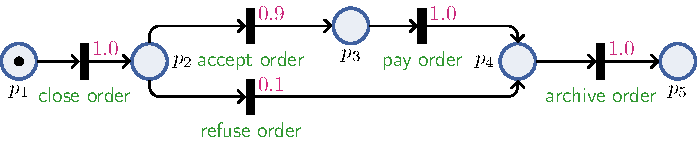
\includegraphics[width=.49\textwidth]{images/petri_tut.pdf}
	\caption{a simple Stochastic Workflow Net.}\label{fig:petri_tut}
	%\vspace{-1.4cm}
\end{figure}
%For example, the probabilistic alignment of a trace with a stochastic net could be represented by the model trace maximizing the combined provision of minimum trace alignment cost and maximum model trace probability. 
With reference to Figure~\ref{fig:petri_tut}, a user might be interested to align the log trace $\langle \textsf{close order},\,\textsf{archive order}\rangle$ with one of the two possible model traces $\langle\textsf{close order},$ $\textsf{accept order},\,\textsf{pay order},\,\textsf{archive order}\rangle$ or $\langle$\textsf{close order}, \textsf{refuse order}, \textsf{archive order}$\rangle$. While the latter trace provides the least alignment cost though the model trace has a low probability ($0.1$), the former gives a slightly greater alignment cost while providing a higher model trace probability ($0.9$). Since, depending on the context, analysts might prefer either the former or the latter alignment, providing a selection of the best $k$ alignments among all the distinct model traces empowers the analysts to find their own trade-off between alignment cost and model trace probability.
%However, in some cases, the user could prefer to identify an alignment with a lower cost even if based on a less probable model trace, while, in other cases, the user could favor a model trace with a higher probability at the expense of a higher alignment cost. Therefore, to provide users with an instrument that allows them to find their own trade-off between alignment cost and model trace probability, we need to return the best $k$ alignments among all the distinct model traces.


%Since when aligning an event log with a stochastic net distinct model traces have different probabilities, the retrieval of the best model trace maximizing the combined provision of minimum trace alignment cost and maximum model trace probability might not suffice. In some cases, indeed, the user could prefer to identify an alignment with a lower cost even if based on a less probable model trace, while, in other cases, the user could favor a model trace with a higher probability at the expense of a higher alignment cost. We consider, therefore, the important tradeoff between both aspects.
%Therefore, in this paper, we propose trace alignment approaches that return the best

To do this, we frame the probabilistic trace alignment problem into the well-known $k$-Nearest Neighbors ($k$NN) problem \cite{Altman} that refers to finding the $k$ nearest data points to a \textit{query}  from a set  of \textit{data points} via a distance function.
We introduce two ranking strategies. The first one is based on a brute force approach that reuses existing trace aligners such as \cite{DBLP:conf/edoc/AdriansyahDA11,LeoniM17}, where the (optimal) ranking of the top-k alignments is obtained by computing the Levensthein distance between the trace to be aligned and all the model traces and by multiplying each of these distances by the probability of the corresponding model trace. However, even if this approach returns the best trace alignment ranking for a query trace, the alignments must be computed a-new for all the possible traces to be aligned. For models generating a large number of model traces, this would clearly become unfeasible. Therefore, we propose a second strategy that produces an approximate ranking where traces are represented as numerical vectors via an embedding. {Then, by exploiting ad-hoc data structures,
	%such as Vp-Trees \cite{Fu2000}, Kd-Trees \cite{Maneewongvatana99}, and M-Trees \cite{Ciaccia},
	we can retrieve the neighborhood of size $k$ containing the traces similar to the given query  by pre-ordering (\textit{indexing}) the model traces  via the aformentioned distance. 
	%Thus, we do not need to analyze the entire space, but just start the search from the top-$1$ alignment. 
	If the embeddings for our model traces are independent of the query of choice, this would not require to constantly recompute the numeric vector representation for the model traces.
	%	
	
	%%%%% Proposed part as the last part of the introduction:
	%\texttt{\color{red}[TODO]}
	%\todo{this is too specific for an introduction; in particular, too many details on how the experiments are done.}
	We implemented both strategies and perform experiments using a real life event log coming from a hospital system to empirically evaluate the properties of our proposed  strategy. We assessed our proposed as follows:
\begin{mylist}
	\item first, we evaluate the degree of approximation introduced by the approximate-ranking approach if compared with the optimal-ranking. We observe that different embedding strategies provide a trade-off between ranking stability vs. precision (\S\ref{subsec:apprp}).
	\item Last, we evaluate the computational time required to both generate the embeddings and to assess the similarity between the embeddings. We observe that approximate-ranking alignments provide the best trade-off between accuracy and efficiency (\S\ref{subsec:efficio}).
\end{mylist}

\begin{figure*}[!t]
	\begin{minipage}{.49\textwidth}
		\centering
		\includegraphics[width=.7\textwidth]{images/petri.pdf}
		\caption{A sample \uswn $N$. Labels are shown in green, $\tau$ transitions in grey, weights in magenta.}\label{fig:spn}
	\end{minipage}\hfill \begin{minipage}{.49\textwidth}
	\centering
		\includegraphics[width=.7\textwidth]{images/rg.pdf}
		\caption{Reachability graph  of the \uswn $N$. Probabilities are shown in violet.}\label{fig:rg}
	\end{minipage}

	\begin{minipage}{.4\textwidth}
		\centering \includegraphics[width=.7\textwidth]{images/running_example.pdf}
		\caption{Preliminary Transition graph $TG$ encoding the SWN $N$ with no $\tau$-closures.}\label{fig:lmc}\label{fig:orig}
	\end{minipage}\hfill \begin{minipage}{.4\textwidth}
	\centering \includegraphics[width=.7\textwidth]{images/closed_example.pdf}
		\caption{Transition graph $TG$ resulting from $N$ after $\tau$-closure.}\label{fig:closed}
	\end{minipage}
	\vspace{-.6cm}
\end{figure*}
\section{Related Works}
%%%
%%%
\paragraph*{Stochastic Conformance Checking} Earlier works on probabilistic trace alignments \cite{AlizadehLZ14a} extended alignment cost functions by considering probabilities that an activity never eventually occurs when activities on both traces do not correspond. Otherwise, such functions always return zero once activity match. This approach favors traces providing optimal alignment: this approach is not ideal for ranking traces, as the resulting ranking provides no trade-off between trace probability and alignment cost. Furthermore, the computation of the aforementioned probability requires the combined provision of a log file and a non-stochastic Petri Net, our proposed solution estimates trace probability by directly assessing Stochastic Petri Nets. After considering that the formers could be always used to estimate the latter \cite{spdwe}, we can deduce that our proposed solution proves to be more general that this first attempt to probabilistic trace alignments. 

More recent works on stochastic model checking \cite{DBLP:conf/icpm/PolyvyanyyK19,DBLP:journals/tosem/PolyvyanyySWCM20} assess the degree of conformance of the whole stochastic model against one single log trace, thus considering the probability distribution of the whole model. On the other hand, we are interested in determining which is the best model trace providing the trade-off between trace probability and alignment cost with the log trace to be aligned, thus limiting the model probability distribution to the part generating one sole given trace at a time. Therefore, such approaches allow to rank models according to the conformance of a give log trace while, on the other hand, our proposed solutions ranks model traces according to one fixed stochastic model. For this reason, we can also reduce our solution to a model rank, while the opposite solution is not possible without changing the overall process distribution. Therefore, our solution is more expressive that the one proposed in current literature.

 
%%%
%%%
\paragraph*{Graph Kernels} Graph kernels express similarity measures \cite{Samatova} involved in both classification \cite{TsudaS10} and clustering algorithms. One of the first approaches required a preliminary embedding definition of topological description vectors extracted from the most frequent subgraphs within a graph database \cite{Sidere}. As a drawback, it required the computation of a subgraph isomorphism problem, which is NP-complete. In fact, the definition of a graph kernel function fully recognizing the structure the graph always boils down to solving such NP-Complete problem \cite{GartnerFW03}, as exact embeddings generable in polynomial can be inferred just for loop-free Direct Acyclic Graphs \cite{BergamiBM20}. Consequently, most recent literature focused on extracting relevant features of such graphs, that are then used to define a graph similarity function. The most common approach adopted in the kernel to extract such features is called \textit{propositionalization}: we might extract all the possible features (e.g., subsequences), and then define a kernel function based on the occurrence and similarity of these features \cite{Gartner03}. For node-labelled graphs, the features come from the node labels and the possible strings that might be generated while traversing the graph (see \cite{Gartner03} and \S\ref{subsec:katk}). 
\section{Foundational Components and Assumptions}
We start by introducing the foundational components of our approach, and the corresponding working assumptions. On the one hand, we describe the class of  Petri nets we consider to represent stochastic processes. On the other hand, we recall graph and string kernels, which we use to compute probabilistic alignments.

\subsection{Stochastic Workflow Nets}\label{subsec:spn}
%As customary in probabilistic conformance checking \cite{DBLP:conf/bpm/LeemansSA19,DBLP:conf/icpm/PolyvyanyyK19,DBLP:journals/tosem/PolyvyanyySWCM20}, we adopt stochastic Petri nets \cite{MarsanCB84,RoggeSoltiAW13} as the underlying formal basis to represent processes. More specifically, we consider an interesting class of stochastic Petri nets with only immediate transitions (i.e., no timed ones).
%We assume to have a set $\alphabet = \tasks \cup \set{\tau}$ of labels, where labels in $\tasks$ indicate process tasks, whereas $\tau$ indicates an invisible execution step ($\tau$-transition). A \emph{trace} is a finite sequence of labels from $\tasks$. An \emph{untimed Stochastic Workflow Net (\uswn)}
%is a tuple $\net = (P,T,F,\ell,W)$ where:
%\textit{(i)} $(P,T,F)$ is a standard \emph{Workflow net} with places $P$, transitions $T$, and flow relation $F$ such that there is exactly one \emph{input place} with no incoming arc, and exactly one \emph{output place} with no outgoing arcs;
%\textit{(ii)} $\ell: T \rightarrow \alphabet$ is a \emph{labeling function} mapping each transition $t \in T$ into a label $\ell(t) \in \alphabet$;
%\textit{(iii)} $W\colon T\to \mathbb{R}^+$ is a \emph{weight function} assigning a positive firing weight to each transition.
%
%\texttt{[TODO: describe the notion of marking]}
%
%By interpreting concurrency by interleaving, we can represent all transition firings of an \uswn, together with their probabilities, in a reachability graph  $(M,E,P)$ where
%\textit{(i)} $M$ is the set of all reachable markings from the initial markings,
%\textit{(ii)} $E \subseteq M \times \alphabet \times M$ is a $\alphabet$-\emph{labeled transition relation} induced by $\net$, that is, for $\marking,\marking' \in M$, we have edge $(\marking,a,\marking') \in E$ if and only if there exists transition $t$ in $\net$ with label $\ell(t) = a$ and such that $\fire{\marking}{t}{\marking'}{\net}$, and
%\textit{(iii)} $P:E \rightarrow [0,1]$ is the \emph{transition probability} function assigning to each transition $(\marking,a,\marking') \in E$ its corresponding probability, obtained from the firing probability of the \uswn transition(s) that lead from $\marking$ to $\marking'$ and are labeled by $a$. 
To model stochastic processes, we isolate an interesting class of Stochastic Petri nets \cite{MarsanCB84,Desel1998,RoggeSoltiAW13}. From the structural point of view, we consider $k$-bounded workflow nets with silent transitions. We assume a set $\alphabet = \tasks \cup \set{\tau}$ of labels, where labels in $\tasks$ indicate process tasks, whereas $\tau$ stands for an invisible execution step ($\tau$-transition). %Labels are associated to transitions via a labelling function $\lambda$.
From the stochastic point of view, do not consider timed aspects, and only focus on the definition of a probability distribution over enabled transitions. We call these nets \emph{stochastic workflow nets} (SWN for short) 
Formally, an SWN is a tuple $\net=(P,T,F,W,i,f)$ where:
\begin{mylist}
	\item $P$ is a set of \textit{places};
	% to which we can associate a finite number of indistinguishable tokens;
	\item $T$ is a set of \textit{transitions} $t\in T$, to which we associate a label $\lambda(t)\in\Sigma$;
	\item $F\subseteq (P\times T)\cup (T\times P)$ is the \emph{flow relation} linking places to transitions and transitions to places; % to which we associate a \textit{firing cost} $\omega\colon F\to\mathbb{N}$;
	\item $W\colon T\to \mathbb{R}$ defines a \textit{firing weight} associated to each transition;
	\item the \emph{initial place} $i\in P$ has no ingoing edges; %($\not\exists t\in T. (t,i)\in F$);
	\item the \emph{final place} $f\in P$ has no outgoing edges. %($\not\exists t\in T. (f,t)\in F$).
\end{mylist}
The notions of marking, transition enablement, transition firing, and reachable markings, are as usual.
%A \textit{marking} is an assignment of a given amount of indistinguishable tokens to places described by a vector $M\colon P\to \mathbb{N}$. We say that a given transition $t$ is \textit{enabled} if $M(p)\geq \omega(p,t)$ for each ingoing $p$ to $t$ ($(p,t)\in F$). If such transition is enabled, then it can \textit{fire} a token. The set of the \textit{enabling transitions} $E(M)$ for a given marking $M$ are all the $t$ reachable from $p$ ($(p,t)\in F$) with $M(p)\neq 0$ where $t$ is enabled. When $t$ can fire a token for a marking $M$, we can generate a novel marking $M'$ from $M$ by moving the tokens from the ingoing places towards the outgoing places as 
%$\forall p\in P.\; M'(p)=M(p)-[\omega(p,t)]+[\omega(t,p)]$. 

We denote by $E(M)$ the set of transitions of $\net$ that are enabled in $M$. Given an initial marking $M$ over $\net$,  the \textit{reachability graph} of $(\net,M)$ is a graph $(\mathcal{M},\mathcal{E})$ with nodes $\mathcal{M}$ and $T$-labelled edges $\mathcal{E}$, where nodes $\mathcal{M}$ are all the reachable markings from $M$ ($M$ included), and where there is an edge from $M$ to $M'$ labeled by $t$ iff $t \in E(M)$ and firing $t$ in $M$ produces $M'$ (this is indicated by $M\overset{t}{\to}M'$).

We consider the two special markings $M_i$ and $M_f$ of $\net$, respectively assigning one token to the initial place $i$ and the final place $f$, and no tokens elsewhere. We say that $\net$ is $k$-\emph{bounded} if each marking in the reachability graph of $(\net,M_i)$ does assigns at most $k$ tokens to each place of $\net$. \emph{As a first, working assumption, we concentrate on $1$-bounded (i.e., safe) nets} (but our technique seamlessly carries over $k$-bounded nets as well).

As usual in stochastic nets, given a marking $M$ we use $W$ to induce a probability distribution over $E(M)$. This is done by assigning to each edge $M\overset{t}{\to}M'$ a corresponding transition probability $\mathbb{P}\left(M\overset{t}{\to}M'\right)=\frac{W(t)}{\sum_{t'\in E(M)}W(t')}$ \cite{spdwe}. Notice that, by construction, the probabilities associated to all enabled transitions in a marking always add up to 1.

A \emph{run} $\seq$ over $\net$ is a finite sequence $t_1\cdots t_n$ of transitions leading from $M_i$ to $M_f$ in the reachability graph of $(\net,M_i)$. The probability $\prob{\seq}{\net}$ of $\seq$ is obtained as as the product of the probabilities associated to each transition via $W$.

\begin{remark}
\label{rem:collective}
The sum of the probabilities of all runs of a SWN, up to a certain maximum length $n$, is always between 0 and 1. When $n$ tends to $\infty$, this sum tends to $1$. This is a direct consequence of how transition probabilities are computed, paired with the fact that runs of a workflow net are maximal.
\end{remark}

%To each of such edges $M\overset{t}{\to}M'$, we associate a transition probability. We say that a SPN with initial marking $M$ is $k$-\textit{bounded} if each of the nodes $M$ in the reachability graph have $\forall p\in P.\; M(p)\leq k$. 

We now turn to traces, defined as finite sequence of labels from $\tasks$ (where each element witnesses the execution of a visible activity). The main issue is that, due to $\tau$-transitions, traces do not directly map into runs. To distinguish model traces from all the possible traces $\tasks^*$, we then proceed as follows. Following \cite{DBLP:conf/edoc/AdriansyahDA11,LeoniM17},  we say that a trace $\nonlogtrace=\const{a}_1\cdots \const{a}_m$ is a \emph{model trace for $\net$} ($\net$-trace for short) if there exists a run $\seq = t_1\cdots t_n$ where the sequence $\lambda(t_1)\cdots \lambda(t_n)$ of labels of $\seq$ coincides with $\nonlogtrace$ once all the $\tau$-labels are stripped away.

There may be multiple, possibly infinitely many runs yielding the same $\net$-trace. Given a $\net$-trace $\nonlogtrace$, we denote by $\seqs{\nonlogtrace}{\net}$ the set of such runs. The probability $\prob{\nonlogtrace}{\net}$ of $\nonlogtrace$ is then obtained by summing up the probabilities of all runs from $\seqs{\nonlogtrace}{\net}$.
This corresponds to the intuition that, to observe $\nonlogtrace$, one can equivalently pick any of its underlying runs. Notably, if a trace is not a $\net$-trace (i.e., it does not conform with $\net$), then its probability is 0. 

To make this probability amenable to computation, we apply a \emph{second working assumption, introduced in \cite{Bergami21}, namely that of bounded silence}. A SWN has \emph{bounded silence} if there exists a fixed bound $b$ limiting the maximum number of consequent $\tau$-transitions between two visible transitions of the run. In \cite{Bergami21}, it is argued that this assumption is reasonable when modeling business processes: it retains the possibility of capturing gateways and skippable tasks, while forbidding whole cycles entirely characterized by $\tau$ transitions, which would in turn generate infinitely many runs yielding the same trace. 

\begin{remark}
\label{rem:silence}
	For a SWN $\net$ with silence bounded by $b$, given a $\net$-trace $\trace$ there are boundedly many runs of $\net$ yielding $\trace$, that is, $\seqs{\nonlogtrace}{\net}$ has a size bounded by $b$, containing runs whose maximum length is bounded by the length of $\trace$ and $b$ \cite{Bergami21}.
\end{remark}

By combining Remarks~\ref{rem:collective} and \ref{rem:silence}, we thus get a direct way of computing the trace probability $\prob{\nonlogtrace}{\net}$.

Since our goal is to handle probabilistic trace alignment, we need to relate a (possibly non-model) arbitrary trace $\logtrace$ over $\tasks^*$ with the most closely $\net$-traces that balance their distance from $\logtrace$ and their probability. In this respect, we notice the following.

\begin{remark}
By increasing the length of $\net$-traces, we reach a point where their probability and distance w.r.t.~the log trace $\trace$ of interest \emph{both} decrease. Intuitively, this is because executing too many loop iterations within $\net$ decreases the overall run probability, and increments the distance to $\trace$.
\end{remark}

Thanks to this final remark, we get that the problem of probabilistic trace alignment works in a finite space of traces and runs, and it is consequently a combinatorial problem that can be attacked with techniques such as $k$-nearest neighbors.



%Our working assumptions are the following: 
%\begin{mylist}
%\item without any loss of generality for concurrent processes, we are interested in 1-bounded SPN, thus allowing an easy conversion from BPMN with no swim-lanes into 1-bounded SPN \cite{RaedtsPUWGS07}.
%\item As customary in trace alignment literature, two traces are equivalent iff. they are identical after stripping $\tau$ events.
%\item As we exploit SPN for generating the traces describing the business process via unfolding, we could discard SPNs containing either \cite{Bergami21}.
%\item Consequently, we could further restrict our analysis to SPNs containing silent transitions representing either skip-able sequences of non-silent transition, or the possibility of choosing different sequences of non-silent transitions \cite{Bergami21}.
%\end{mylist} We refer to a SPN satisfying such constraints as \textsc{Stochastic Workflow Nets} (SWN). 




%\todo[inline]{Non capisco la frase}
%Given a log trace $\logtrace$ coming from a log file $\mathcal{L}$, we always associate to it a certain probability, i.e., $\prob{\logtrace}{\mathcal{L}}=1$. 





%\begin{definition} An \emph{untimed Stochastic Workflow Net (\uswn)}
%	is a tuple $\net = (P,T,F,\ell,W)$ where:
%	\begin{inparaenum}[\itshape (i)]
%		%\begin{inparaenum}
%		\item $(P,T,F)$ is a standard \emph{Workflow net} with places $P$, transitions $T$, and flow relation $F$ such that there is exactly one \emph{input place} with no incoming arc, and exactly one \emph{output place} with no outgoing arcs;
%		\item $\ell: T \rightarrow \alphabet$ is a \emph{labeling function} mapping each transition $t \in T$ into a label $\ell(t) \in \alphabet$ - this either indicates the task executed upon firing $t$, or the fact that $t$ is an invisible transition (in the latter case, $\ell(t) = \tau$);
%		\item $W\colon T\to \mathbb{R}^+$ is a \emph{weight function} assigning a positive firing weight to each transition of the net.
%	\end{inparaenum}
%\end{definition}
%Given an \uswn $\net$, we use dot notation to extract its constitutive components (e.g., $\net.P$ denotes its places). \emph{The same dot notation will be used for the other structures introduced in the paper}. We also use $\net.in$ and $\net.out$ to respectively denote the input and output place of $\net$.
%The current state of execution is captured by a marking, i.e., a multiset of places $P$ indicating how many tokens populate each place.
%As pointed out above, \emph{we always assume, as customary in BPM, that the input \uswn is \underline{bounded}}, that is, in every state the number of tokens associated to each place cannot exceed a maximum, fixed threshold.
%The notions of transition enablement and firing are also the standard ones  \cite{MarsanCB84}, as well as the ones for \textit{firing probability} \cite{spdwe}. %: %, which provides the basis for capturing the stochastic behavior of the net. 
%We use the following notation: given a marking $\marking$ over \uswn $\net$,  $\enaset{\marking}{\net}$ is the set of enabled transitions in $\marking$; given transition $t \in \enaset{\marking}{\net}$, we write $\fire{\marking}{t}{\marking'}{\net}$ to capture the fact that, with, firing $t$ in $\marking$ results in the new marking $\marking'$. A \emph{firing sequence starting from marking $\marking_0$} is a sequence $t_1\cdots t_n$ of transitions from $\net.T$ so that, for every $i \in \set{1,\ldots,n}$, we have that $\fire{\marking_{i-1}}{t_i}{\marking_{i}}{\net}$. We say that the firing sequence results in $\marking_{n}$.
%
%given a marking $\marking$ %of $N$ 
%and an enabled transition $t \in T_e$, the \emph{firing probability} of $t$ in $\marking$ is $\probt{t}{\marking}{\net} = \frac{W(t)}{\sum_{t'\in T_e}W(t')}$. %As required, 


%A \emph{valid sequence} $\seq = t_1\cdots t_n$ is a firing sequence starting from $m_{in}$ and resulting in $m_{out}$. The probability $\prob{\seq}{\net}$ of a valid sequence is the product of the probabilities associated to each transition. %: $\prob{\seq}{\net} = \prod_{i \in \set{1,\ldots,n}}\prob{t_i}{\marking_{i-1},\net}$. % A sequence of labels $\run = \alpha_1 \cdots \alpha_n$ from $\alphabet$ is a \emph{run} if there exists a valid underlying sequence $\seq = t_1\cdots t_n$  having $\alpha_i$ as a label for each $t_i\in \seq$. Run $\run$ may have different underlying valid sequences in $\seqs{\run}{\net}$.

%underlying run $\run$ corresponding to $\trace$ once all $\tau$ are removed. 

\subsection{Graph and String Kernels}\label{subsec:katk}
 As a foundational basis to compute trace alignments, we adapt similarity measures from the database literature.  Given a set of data examples $\mathcal{X}$, (e.g., strings or traces, transition graphs) a (positive definite) \emph{kernel} function $k\colon \mathcal{X}\times \mathcal{X}\to \mathbb{R}$ denotes the similarity of elements in $\mathcal{X}$. If $\mathcal{X}$ is the $d$-dimensional Euclidean Space $\mathbb{R}^d$, the simplest kernel function is the inner product $\Braket{\mathbf{x},\mathbf{x}'}=\sum_{1\leq i\leq d}\mathbf{x}_i\mathbf{x}'_i$.
A kernel is said to \emph{perform ideally} \cite{Gartner03} when $k(x,x')=1$ whenever $x$ and $x'$ are the same object (\textit{strong equality}) and $k(x,x')=0$ whenever $x$ and $x'$ are distinct objects (\textit{strong dissimilarity}). A kernel is also said to be \emph{appropriate} when similar elements $x,x'\in\mathcal{X}$ are also close in the feature space. Notice that appropriateness can be only assessed  empirically \cite{Gartner03}.
A positive definite kernel induces a distance metric as 
$
d_k(\mathbf{x},\mathbf{x}'):=\sqrt{k(\mathbf{x},\mathbf{x})-2k(\mathbf{x},\mathbf{x}')+k(\mathbf{x}',\mathbf{x}')}
$.
When the kernel of choice is the inner product, the resulting distance is the Euclidean distance $\norm{\mathbf{x}-\mathbf{x}'}{2}$. A normalized vector $\hat{\mathbf{x}}$ is defined as $\mathbf{x}/\norm{\mathbf{x}}{2}$. For a normalized vector we can easily prove that: $\norm{\hat{\mathbf{x}}-\hat{\mathbf{x}}'}{2}^2=2(1-\Braket{\hat{\mathbf{x}},\hat{\mathbf{x}}'})$.
When $\mathcal{X}$ does not represent directly a $d$-dimensional Euclidean space, we can use an \emph{embedding} $\embed\colon\mathcal{X}\to \mathbb{R}^d$ to define a kernel $k_\embed\colon \mathcal{X}\times \mathcal{X}\to\mathbb{R}$ as $k_\embed(x,x'):=\Braket{\embed(x),\embed(x')}$. As a result, $k_\embed(x,x')=k_\embed(x',x)$ for each $x,x'\in\mathcal{X}$.



 The literature also provides a kernel representation for strings \cite{LodhiSSCW02,GartnerFW03}: if we associate each dimension in $\mathbb{R}^d$ to a different sub-string $\alpha\beta$ of size $2$ (i.e., $2$-grams\footnote{\label{fn:caveat}For our experiments, we choose to consider only $2$-grams, but any $p$-grams of arbitrary length $p\geq 2$ might be adopted \cite{Gartner03}. An increased size of $p$ improves precision but also incurs in a worse computational complexity, as it requires to consider all the arbitrary subtraces of length $p$ whose constitutive elements occur at any distance from each other within the trace.}), it should represent how frequently and ``compactly'' this subtrace is embedded in the trace $\trace$ of interest. Therefore, we introduce a \emph{decay factor} $\lambda\in[0,1]\subseteq\mathbb{R}$ that, for all $m$ sub-strings where $\alpha$ and $\beta$ appear in $\trace$ at the same relative distance $l < |\trace|$, weights the resulting embedding as $\lambda^lm$.



\begin{table*}[t!]
	\vspace{+0.7cm}
	\caption{Embedding of traces $\const{caba}$, $\const{caa}$ and $\const{cb}$.}\label{tb:embedding}
	\vspace{-0.4cm}
	\begin{center}
		%\scalebox{0.6}
		{
			\begin{tabularx}{\textwidth}{
					>{\hsize=.1\hsize}X
					>{\hsize=.2\hsize}X
					>{\hsize=.1\hsize}X
					>{\hsize=.1\hsize}X
					>{\hsize=.1\hsize}X
					>{\hsize=.1\hsize}X
					>{\hsize=.1\hsize}X
					>{\hsize=.25\hsize}X
					>{\hsize=.2\hsize}X
					>{\hsize=.1\hsize}X
				}
				\toprule
				& $\const{aa}$    & $\const{ab}$   & $\const{ac}$    & $\const{ba}$   & $\const{bb}$   & $\const{bc}$ & $\const{ca}$ & $\const{cb}$ & $\const{cc}$   \\
				\midrule
				$\const{caba}$ & $\lambda^2$ & $\lambda$ & $0$ & $\lambda$  & $0$  & $0$ & $\lambda+\lambda^3$ & $\lambda^2$ & $0$\\
				%$\const{caaa}$ & $2\lambda+\lambda^2$& $0$ & $0$ & $0$ & $0$ & $0$ & $\lambda+\lambda^2+\lambda^3$ & $0$ & $0$ \\
				$\const{caa}$  & $\lambda$ & $0$ & $0$ & $0$ & $0$ & $0$ & $\lambda+\lambda^2$ & $0$&  $0$\\
				$\const{cb}$   & $0$ & $0$ & $0$ & $0$ & $0$ & $0$ & $0$ & $\lambda$& $0$ \\
				\bottomrule
			\end{tabularx}
		}
		\vspace{-0.3cm}
	\end{center}
\end{table*}
\begin{example}\label{ex:wheredotiszero} %\small
	Consider tasks $\tasks=\Set{a,b,c}$. The possible 2-grams over $\tasks$ are $\tasks^2=\Set{\const{aa},\const{ab},\const{ac},\const{ba},\const{bb},\const{bc},\const{ca},\const{cb},\const{cc}}$. Table~\ref{tb:embedding} shows the embeddings of some traces. Being a 2-gram, trace $\const{cb}$ has only one nonzero component, namely that corresponding to itself, with $\trembed_{\const{cb}}(\const{cb})=\lambda$. Trace $\const{caa}$ has the 2-gram $\const{ca}$ occurring with length $1$ ($\const{\underline{ca}a}$) and $2$ ($\const{\underline{c}a\underline{a}}$), and the 2-gram $\const{aa}$ with occurring length $1$ ($\const{c\underline{aa}}$). Hence: $\trembed_{\const{ca}}(\const{caa})=\lambda+\lambda^2$ and  $\trembed_{\const{aa}}(\const{caa})=\lambda$.  Similar considerations can be carried out for the other traces in the table.
	We now want to compute the similarity between the first trace $\const{caba}$ and the other two traces. To do so, we sum, column by column (that is, 2-gram by 2-gram) the product of the embeddings for each pair of traces. We then get $k_{\trembed}(\const{caba},\const{caa})=\lambda^3+(\lambda+\lambda^3)(\lambda+\lambda^2)$ and $k_{\trembed}(\const{caba},\const{cb})=\lambda^3
	$,
	%{\footnotesize
	%\[
	%k_{\trembed}(\const{caba},\const{caaa})=\lambda(\lambda+\lambda^2+\lambda^3)
	%~~
	%k_{\trembed}(\const{caba},\const{caa})=\lambda(\lambda+\lambda^2)
	%~~
	%k_{\trembed}(\const{caba},\const{cb})=\lambda(\lambda+\lambda^3)
	%\]}
	which induces ranking $
	k_{\trembed}(\const{caba},\const{caa})>
	k_{\trembed}(\const{caba},\const{cb})
	$.
\end{example}

Nevertheless, such string embedding has several shortcomings: \begin{alphalist}
	\item it is not weakly-ideal, so we cannot numerically assess if two embeddings represent equivalent traces 
	(Example \ref{ex:wheredotiszero});
	\item it does not characterize $\tau$-moves, so the probabilities of the initial and final $\tau$-moves are not preserved; and
	\item it is affected by numerical errors from finite arithmetic: longer traces $\nonlogtrace$ generated from skewed probability 
	distributions %$G.\Lambda^i$
	yield greater truncation errors, as smaller $\lambda^i$ components for bigger 
	$i<|\nonlogtrace|$ are ignored, preventing a complete numerical vector characterization of  $\nonlogtrace$ in practice.
\end{alphalist}

\endinput





\section{Working Assumptions}\label{sec:was}
%We assume that the model against which we want to align the log traces is fixed as in previous papers exploiting database technologies for business process management techniques \cite{SchonigRCJM16}. Therefore, we always assume to know all the traces associated to a procedural model, as well as their associated probabilities \cite{AlizadehLZ14a}. As we will show in the next section, this assumption will make the alignment process more efficient, as we can focus efficiently aligning multiple log traces.

%This section shows that, 
%starting from common assumptions from the BPM community, we are able to transform reachability graphs into a node-labeled Markovian Process, where  $R$ is the associated transition matrix and $L$ is the node-labeling matrix. In fact, such matrices can determine the probability of reaching a node labeled $\beta\in\Sigma$ from any node labelled $\alpha\in\Sigma$ in $n$ steps as in string kernels:   $[\Lambda^n]_{\alpha\beta}:=[LR^nL^\top]_{\alpha\beta}/[LL^\top]_{\alpha\alpha}$ (see \cite{GartnerFW03} and Example \ref{ex:wheredotiszero}).
%

%As a first result, the set of all the traces generated from the unfolding of SWN partition the sample space. This is the result of the two following considerations: \begin{mylist}
%\item Given the requirements over the initial and final markings, we will generate a reachability graph $(\mathcal{M},\mathcal{E})$ where the initial (final) marking has no ingoing (outgoing) edges;
%\item also, by definition of the transition probability, the sum of the transition probabilities from a marking $M$ towards the adjacent $M'$ always adds up to $1$.
%\end{mylist}

%Finally, we can intuitively prove the goal asserted at the beginning of the current section: 
%first, we need to shift labels from edges to nodes, and then we perform $\tau$-closures while preserving (if required) $\tau$-transitions for both start and final nodes; such operations preserve the traces' probabilities \cite{Bergami21}. Next, the transition probabilities are going to be stored in a matrix $R$ representing a stochastic process, while for each node $i$ there is only one label $\alpha$ such that $[L]_{i\alpha}=1$, and $[L]_{i\beta}=0$ if $\alpha\neq\beta$. Therefore, runs for Markovian Processes are then defined as for SWNs, and we employ the same notation to indicate the valid sequences underlying a model trace. The computation of probabilities for traces is hence defined equivalently. We denote these pair of matrices as \textsc{Transition Graph} $TG=(L,R)$.

\endinput
Petri Nets and Generalized Stochastic Petri Nets are well-established formalisms \cite{DBLP:journals/tosem/PolyvyanyySWCM20} for modelling processes \cite{RoggeSoltiAW13} represented in the Petri Net Markup Language, supported by our tool. Due to the lack of space, we refer to \cite{spdwe} for the usual notation over Petri Nets. We restrict our interest to an interesting class of $1$-\textit{bounded} stochastic Petri nets with no timed transitions, namely \textsc{untimed Stochastic Workflow Nets} denoted as $N$. We now sketch the properties of the SWN sketched in \cite{Bergami21}. We consider a single \emph{input} (\emph{output}) marking $m_{in}$ ($m_{out}$) assigning a single token to the input (output) place, and no token elsewhere [\dots].


[\dots] These structural properties makes them suitable for converting BPMN models with no swim-lanes as SWN, which firing weight could be estimated from their associated log files \cite{spdwe}.
\begin{example} %\small
	\label{ex:net}
	\figurename~\ref{fig:spn} shows an example of an \uswn with input place $p_1$ and output place $p_7$. One run of the net is $\const{\tau c \tau a a \tau}$, which corresponds to trace $\const{caa}$. Overall, the net supports infinitely many finite traces of the form (represented using regular expressions):
	\begin{inparaenum}[\it (i)]
		\item $\const{aa^*}$,
		\item $\const{cb}$,
		\item $\const{caa^*}$.
	\end{inparaenum}
\end{example}
%When executing an \uswn, the crucial addition to the standard execution semantics of Workflow nets is that, being the net stochastic, in each marking the set of enabled transitions gets associated to a discrete probability distribution. This is defined as follows:
%given a marking $\marking$ of $N$ and an enabled transition $t \in \enaset{\marking}{\net}$, the \emph{firing probability} of $t$ in $\marking$ is $\probt{t}{\marking}{\net} = \frac{\net.W(t)}{\sum_{t'\in \enaset{\marking}{\net}}\net.W(t')}$. As required, the probabilities associated to all enabled transitions in a marking always add up to 1.
% %For a run $\run$ of $\net$, its probability $\prob{\seq}{\net}$ is then obtained by summing up the probabilities of all valid sequences corresponding to $\run$: $\prob{\run}{\net} = \sum_{\seq \in \seqs{\run}{\net}} \prob{\seq}{\net}$. Likewise, for a trace $\trace$ of $\net$, its probability is obtained by summing up
% For convenience, when needed, we represent an $\net$-trace as a pair $\tup{\trace,\prob{\trace}{\net}}$, where the probability assigned to $\trace$ by $\net$ is retained.

We need to lift this approach so as to consider all occurrences of subtraces $\alpha\beta$ at every distance between $1$ and $|\trace|-1$. To do so, we proceed in two steps. First, we encode $\trace$ into a ``linear'' transition graph $\tg_\trace$ (\figurename~\ref{fig:taustar}) in the obvious way. %\todo{Tagliare dopo i due punti se necessario.} each node in $G_\sigma.V$  corresponds to an element of the trace labeled correspondingly, and the nodes representing two consecutive elements in the trace are connected with a transition probability of 1 (whereas in all the other cases, the probability is 0).
As a second step, we rely on the matrix operations to calculate a simplified version of the embedding defined in \cite{LodhiSSCW02} as $\trembed_{\alpha\beta}(\trace)=\sum_{1\leq i\leq |\trace|}\lambda^i[(\tg_{\trace}.\Lambda)^i]_{\alpha\beta}$. %\todo{No spazio per spiegare cosa succede...}
%This value can be seen as a reward.
The kernel between two traces corresponds to the sum of the products of such values calculated 2-gram by 2-gram for the two traces.
%, namely it is equal to the \emph{kernel convolution}. %\todo{L'ho provato a scrivere intuitivamente, ma non e' chiaro da dove arrivi questo modo di calcolarlo... deriva dalle formule sopra ma la digressione in mezzo e' lunga. Come possiamo fare per chiarire? L'esempio spiega bene tutto!}
This trace kernel returns strong dissimilarity when the two traces have no shared 2-grams at any arbitrary occurring length, but does not enjoy strong equality (as the similarity of a trace with itself is at least $\lambda^2$ - returned when the trace is a 2-gram).

%
%we can represent it as a TG \cite{Myers1989} $(1,{|\tau|},L_\tau,R_\tau,1)$ having $[L_\tau]_{{\color{green}\alpha}\texttt{\color{blue}i}}=1\Leftrightarrow \tau_{\texttt{\color{blue}i}}={\color{green}\alpha}$ and $[L_\tau]_{{\color{green}\alpha}\texttt{\color{blue}i}}=0$ otherwise, and $\forall i<|\tau|.\; [R_\tau]_{\texttt{\color{blue}i(i+1)}}=1 $ and $[R_\tau]_{\texttt{\color{blue}ij}}=0$ otherwise.
%Exploiting this encoding, we can adopt a simplified version of the embedding defined in \cite{LodhiSSCW02,Raedt} as $\embed_{\mathcal{T}}(\tau)_{{\color{green}\alpha\beta}}=\sum_{1\leq i\leq |\tau|}\lambda^i[(\Lambda_\tau)^i]_{\color{green}\alpha\beta}$.
%Please note that this definition is similar to a transition matrix embedding proposed in \cite{GartnerFW03} via geometric series, that is $\sum_i\lambda^i[R^i]_{\color{green}\alpha\beta}$.

\begin{figure}[!t]
	\centering
	\includegraphics[width=.4\textwidth]{images/taustar.pdf}
	\caption{Graphical representation of the transition graph encoding trace $\const{caba}$.}\label{fig:taustar}
	
\end{figure}
%
%\begin{example}\label{ex:tracembed}
%	{Let us suppose that we want to align a trace $\tau^*$ to one of the traces from a transition graph: in order to carry out an approximate alignment, we need to transform it to a transition graph first.} A trace $\tau^*=\textup{caba}$ can be graphically represented in Figure \ref{fig:taustar}. The associated TG $T=(\mathtt{\color{blue}1},\mathtt{\color{blue}4},L,R,1)$ has matrices $L$ and $R$  defined as follows:
%	$$L:=\kbordermatrix{
%		& \texttt{\color{blue}1}&\texttt{\color{blue}2}&\texttt{\color{blue}3}&\texttt{\color{blue}4}\\
%		\color{green}a            & 0&\textbf{1}&0&\textbf{1}\\
%		\color{green}b            & 0&0&\textbf{1}&0\\
%		\color{green}c            & \textbf{1}&0&0&0\\
%	}\qquad R:=\kbordermatrix{
%		& \texttt{\color{blue}1}&\texttt{\color{blue}2}&\texttt{\color{blue}3}&\texttt{\color{blue}4}\\
%		\texttt{\color{blue}1}  & 0&\color{red}1&0&0\\
%		\texttt{\color{blue}2}  & 0&0&\color{red}1&0\\
%		\texttt{\color{blue}3}  & 0&0&0&\color{red}1\\
%		\texttt{\color{blue}4}  & 0& 0& 0& 0\\
%	}$$
%We can similarly represent all the traces from the USPN.
%\end{example}

%\begin{example}
%The subtrace \textit{\textbf{\uline{hi}}} is represented in \textit{\textbf{\uline{hi}}deous},   \textit{\uline{\textbf{h}}e\uline{{i}}d\textbf{i}}, and \textit{\uline{{\textbf{h}i}}nd\textbf{i}}, but with different frequencies and subtrace distances. We have $\embed_{\mathcal{T}}(\textit{hideous})_{{\color{green}hi}}=\lambda$,  $\embed_{\mathcal{T}}(\textit{heidi})_{{\color{green}hi}}=\lambda^2+\lambda^4$, and $\embed_{\mathcal{T}}(\textit{hindi})_{{\color{green}hi}}=\lambda+\lambda^4$.
%\end{example}


%\begin{figure*}[!t]
	\begin{minipage}{.49\textwidth}
		\centering
		\includegraphics[width=.7\textwidth]{images/petri.pdf}
		\caption{A sample \uswn. Labels are shown in green, $\tau$ transitions in grey, weights in magenta.}\label{fig:spn}
	\end{minipage}\hfill \begin{minipage}{.49\textwidth}\centering
		\includegraphics[width=.8\textwidth]{images/rg.pdf}
		\caption{Reachability graph $RG(N)$ of the \uswn $N$. Probabilities are shown in violet.}\label{fig:rg}
	\end{minipage}
\end{figure*} \begin{figure*}[!t]
	\begin{minipage}{.49\textwidth}\centering \includegraphics[width=.55\textwidth]{images/running_example.pdf}
		\caption{Transition graph $G_{RG(N)}$ encoding the reachability graph $RG(N)$.}\label{fig:lmc}\label{fig:orig}
	\end{minipage}\hfill \begin{minipage}{.49\textwidth}\centering \includegraphics[width=.55\textwidth]{images/closed_example.pdf}
		\caption{Transition graph $\closed{G_{RG(N)}}$ resulting from the transition graph in $G_{RG(N)}$ after $\tau$-closure.}\label{fig:closed}
	\end{minipage}
\end{figure*}
\section{Computation Pipeline}
%\begin{figure}[!t]
%	\centering
%	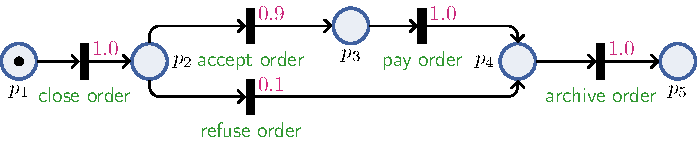
\includegraphics[width=.49\textwidth]{images/petri_tut.pdf}
%	\caption{Stochastic Workflow Net modeling our use-case scenario.}\label{fig:petri_tut}
%\end{figure}
\begin{figure}[!t]
	\centering\includegraphics[width=\textwidth]{images/pipeline}
	\caption{Proposed pipeline to assess the probabilistic trace alignment.}\label{fig:pipe}
\end{figure}

%We now describe the proposed technique for computing probabilistic trace alignments. 
Our approach (\figurename~\ref{fig:pipe}) takes as input
\begin{inparaenum}[\it (i)]
	\item a reference model represented as Stochastic Workflow Nets $\net$ or an equivalent Transition Graph $G$,
	\item a minimum, positive probability threshold $\pmin \in (0,1]$
	\item a trace $\trace$ of interest,
\end{inparaenum}
and returns a ranking over all the $\net$-traces having a probability greater than or equal to $\pmin$, based on a combined consideration of their probability values and their distance to $\trace$.
\section{Alignment Strategy}\label{subsec:as}

Starting from common assumptions from the BPM community, we are able to transform reachability graphs into a node-labeled Markovian Process, where  $R$ is the associated transition matrix and $L$ is the node-labeling matrix. In fact, such matrices can determine the probability of reaching a node labeled $\beta\in\Sigma$ from any node labelled $\alpha\in\Sigma$ in $n$ steps as in string kernels:   $[\Lambda^n]_{\alpha\beta}:=[LR^nL^\top]_{\alpha\beta}/[LL^\top]_{\alpha\alpha}$ (see \cite{GartnerFW03} and Example \ref{ex:wheredotiszero}).
%

first, we need to shift labels from edges to nodes, and then we perform $\tau$-closures while preserving (if required) $\tau$-transitions for both start and final nodes; such operations preserve the traces' probabilities \cite{Bergami21}. Next, the transition probabilities are going to be stored in a matrix $R$ representing a stochastic process, while for each node $i$ there is only one label $\alpha$ such that $[L]_{i\alpha}=1$, and $[L]_{i\beta}=0$ if $\alpha\neq\beta$. Therefore, runs for Markovian Processes are then defined as for SWNs, and we employ the same notation to indicate the valid sequences underlying a model trace. The computation of probabilities for traces is hence defined equivalently. We denote these pair of matrices as \textsc{Transition Graph} $TG=(L,R)$.


When aligning a log trace with a TG, retrieving the model trace maximizing the combined provision of minimum trace alignment cost
and maximum model trace probability does not suffice.
Hence, we find the best $k$ alignments among all  model traces in $\ptraces{\net}{\pmin}$. This reduces to the
$k$-nearest neighbors ($k$NN) problem by finding the $k$ nearest data points to a \textit{query} $x$ from a set
$\mathcal{X}$ of \textit{data points} w.r.t.\ a given distance function $d_k$. Through ad-hoc data structures, such as VP-Trees
and KD-Trees, %VP-Trees \cite{Fu2000} \cite{Maneewongvatana99}, and M-Trees \cite{Ciaccia},
we can retrieve the $k$-neighborhood of $x$ in $\mathcal{X}$ by pre-ordering (\textit{indexing}) $\mathcal{X}$ with respect to $d_k$.
%and searching from the top-$1$ alignment.
%
%To align a trace $\logtrace$ over the \unravelled\ traces $\ptraces{\tg}{\pmin}$,
%the $k$-Nearest Neighbors describe the best $k$ alignments for $\logtrace$.
%We discuss two strategies to obtain these
%alignments.

\smallskip
\noindent
\textbf{Optimal-Ranking Trace Aligner.}
One approach is to reuse existing trace aligners and compute the alignment cost for each model trace $\nonlogtrace$ to be aligned with a model trace at a time $\logtrace$. Customary alignments \cite{DBLP:conf/edoc/AdriansyahDA11,LeoniM17} can be efficiently computed via string Levenshtein distance $d(\logtrace,\nonlogtrace)$: therefore, we will consider traces as strings with associated probability values. Given that similarity is the inverse function of distance and that, concerning the alignment task, we want to find the model trace maximizing both probability and similarity with the log trace, the problem boils down to maximizing the product $p\cdot s$, where $p=\prob{\logtrace}{\mathcal{L}}\prob{\nonlogtrace}{\net}=\prob{\nonlogtrace}{\net}$ and $s=\frac{1}{\frac{1}{c}d(\logtrace, \nonlogtrace)+1}$, where $c\in\mathbb{N}_{\neq 0}$ is a constant. We refer to $p\cdot s$ as the golden ranking function denoted as $\mathcal{R}(\logtrace,\nonlogtrace)$.


%Using decision theory \cite{dectheor}, we express the ranking score as the product
%$\probskip{\nonlogtrace} d(\logtrace,\nonlogtrace)$, taking into account the cost of the alignment (the distance between
%the model trace and the trace to be aligned) and the probability of the model trace.
%
%To represent the same intuition of a weighted distance as a ranking function, we transform it into a
%similarity function returning $1$ when $\nonlogtrace=\logtrace$ and $\probskip{\logtrace}=1$ hold. We express $d$ as
%a normalized similarity score $s_d(\logtrace,\nonlogtrace):=\frac{1}{\frac{1}{c}d(\logtrace,\nonlogtrace)+1}$, where
%$c\in\mathbb{N}_{\neq0}$ is a constant. The maximum similarity is reached when the distance is $0$ and the similarity decreases
%as the distance increases.
%The golden ranking function producing the optimal ranking is
%$\goldenrank(\logtrace,\nonlogtrace)=\probskip{\nonlogtrace} \probskip{\logtrace} s_d(\logtrace,\nonlogtrace)$;
%${\max\arg}_{\nonlogtrace\in \WCal{\pmin}{n}} \goldenrank(\logtrace,{\nonlogtrace})$ yields the best optimal-ranking trace
%alignment for a log trace $\logtrace$, where $\goldenrank$ must be computed anew for each possible $\logtrace$.
%{We can represent each trace as a point  $(\mathbb{P}_N(\sigma)\mathbb{P}_N(\sigma'),\; s_d(\sigma,\sigma'))$ in the
%	2-dimensional similarity/probability space of coordinates $(p,s)$, reducing the trace finding problem to maximising the product
%	$p\cdot s\equiv \mathbb{P}_N(\sigma)\mathbb{P}_N(\sigma')\cdot s_d(\sigma,\sigma')$ (Figure \ref{fig:sps}).}
%
%\begin{figure}[!t]
%	\centering
%	\vspace{-4mm}
%	\subfloat{\label{fig:spp}\includegraphics[width=.5\textwidth]{images/original_space.pdf}}
%	\subfloat{\label{fig:knnspace}\includegraphics[width=.5\textwidth]{images/transformed_space.pdf}}\\
%	\caption{Two characterizations of probabilistic trace alignment; the similarity/probability space left, and the transformed
%		$k$NN space right. The best possible match is shown in red in both spaces.}\label{fig:sps}
%\end{figure}


\begin{table}[!t]
	\vspace{5mm}
	\centering
	\caption{Golden ranking of model traces with maximum length $4$, where $\logtrace=\const{caba}$ and $c=5$.}\label{tab:expected}
	\resizebox{.45\textwidth}{!}{\begin{tabular}{lc|ll|c}
			\toprule
			
			{$\nonlogtrace$} &
			{$d(\sigma',\sigma)$} &
			$( \mathbb{P}_N(\sigma')$ &  $,\,s_d(\sigma',\sigma)) $ &
			{$\approx s_d(\sigma,\sigma^*)\cdot w_\sigma$} \\
			
			
			\midrule
			$\const{a}$  & $3$ & $0.4$ & $\;\; 0.6250$  & $0.2500$\\
			$\const{aa}$  & $2$ & $0.2$ & $\;\; 0.7142$ & $0.1428$\\
			$\const{aaa}$  & $2$ & $0.1$ & $\;\; 0.7142$ & $0.0714$ \\
			$\const{ca}$  & $2$ & $0.07$ & $\;\; 0.7142$ & $0.0500$\\
			$\const{cb}$  & $2$ & $0.06$ & $\;\; 0.7142$ & $0.0428$ \\
			$\const{aaaa}$  & $3$ & $0.05$ & $\;\; 0.7142$ & $0.0357$ \\
			$\const{caa}$  & $1$ & $0.035$ & $\;\; 0.8333$ & $0.0292$ \\
			$\const{caaa}$  & $1$  & $0.0175$ & $\;\; 0.8333$ & $0.0145$ \\
			\bottomrule
	\end{tabular}}
\end{table}
\begin{example}\label{ex:rankingTaus}
	Consider the TG $\closed{\tg}$ in \figurename~\ref{fig:lmc} with probabilities
	$\pa=0.8$, $\pb=0.2$, $\pc=\pf=0.5$, $\pd=0.7$, and $\pe=0.3$. The traces with maximum length $4$ are:
	%$$\begin{aligned}
	%\ptraces{\expN}{0}_{|\nonlogtrace|\leq 4}=
	$\{\braket{\const{a},0.4},\braket{\const{aa},0.2}$, $\braket{\const{aaa},0.1}$, $\braket{\const{ca},0.07}$,
	$\braket{\const{cb},0.06}$,
	$\braket{\const{aaaa},0.05},\braket{\const{caa},0.035},\braket{\const{caaa},0.0175}\}$.
	Table \ref{tab:expected} represents their alignment raking with  $\nonlogtrace=\textup{caba}$.  Although $\const{caa}$ and
	$\const{caaa}$ are the most similar to $\const{caba}$, their associated probability  is rather low, so traces with
	higher probability but lower similarity score are preferred (e.g., $\const{a}$ and $\const{aa}$).
\end{example}
%
{Since users might still prefer the most similar traces to the ones maximizing both probability and similarity, we
	return the best $k$ solutions.
	We reduce the problem to $k$NN over the Euclidean Space through a transformation $t$ such that the distance of the
	transformed point $t(p,s)$ from  the origin $\vec{0}$ is $\sfrac{1}{ps}$. This preserves the score from the golden ranking
	and maps the points maximizing $ps$ close to the origin, but it requires to recompute the transformation for each new log trace $\logtrace$. We choose}
$t(p,s):=\left(\frac{1}{s\sqrt{p^2+s^2}},\; \frac{1}{p\sqrt{p^2+s^2}}\right)$.
Our search always starts from the origin, and hence finds the best candidates first.
%
%\begin{example}
	{Given a family of hyperbolae $p\cdot s$ with all the alignments having
		$\mathcal{R}(\sigma,\sigma')=p\cdot s$.
%		Point $(1,1)$ is the best possible trace match, i.e., a trace
%		$\nonlogtrace\in\ptraces{G}{0}$ with $\nonlogtrace=\logtrace$ and $\mathbb{P}_G(\nonlogtrace)\mathbb{P}_G(\logtrace)=1$.
%		%		
%		Figure \ref{fig:knnspace} (below) shows that
%		
	the embedding moves the points of the hyperbola $p\cdot s$ to a circumference $x^2+y^2=\sfrac{1}{(ps)^2}$ describing a locus of the points equidistant as $\sfrac{1}{ps}$ from the origin of the axes $(0,0)$.}
%\end{example}
%
The transformation required for running the $k$NN algorithm preserves the golden ranking.

\begin{lemma}
	\label{lem:transfspace}
	The set of points having the product $ps$ at least $k\in[0,1]$ corresponds to the set of $t$-transformed points with distance
	at least $1/k$ from the origin.
\end{lemma}

\noindent
\textbf{Approximate-Ranking Trace Embedder.}\label{subsec:ate}
Ranking optimality comes at the cost of a brute-force recomputation of $\goldenrank$ for each trace $\logtrace$ to align. Alternatively, we might avoid the brute-force cost by
%Each embedding $\phi$ entails an associated similarity metric $k_\phi$ (\S\ref{subsec:katk}) and an associated
%distance $d_{k_\phi}$ (Equation \ref{eq:dofk}), hence
%we can compute
computing the embeddings for all the \unravelled\ traces
before the top-$k$ search ensuring that they are independent of the trace to align. %, avoiding the brute-force cost.
%As previously observed,
This computational gain comes with a loss in precision, that our embedding proposal tries to mitigate by overcoming some of the current literature shortcomings:
%; the generation of precise embeddings for graph data with loops is
%NP-complete \cite{GartnerFW03}. %and, in its approximated version, is unable to accurately represent data using low-dimensional
%%vectors \cite{Seshadhri5631}.
%Our proposed embedding ($\gorgembed$) is thus weakly-ideal (\S\ref{subsec:katk}).
%%
%$\gorgembed$ is a variant of the embedding $\trembed$ from \cite{LodhiSSCW02}, which addresses some of its shortcomings.
%Indeed, $\trembed$
%\begin{alphalist}
%	\item is not weakly-ideal, so we cannot numerically assess if two embeddings represent equivalent traces
%	(Example \ref{ex:wheredotiszero});
%	\item does not characterize $\tau$-moves, so the probabilities of the initial and final $\tau$-moves are not preserved; and
%	\item is affected by numerical errors from finite arithmetics: longer traces $\nonlogtrace$ generated from skewed probability
%	distributions $G.\Lambda^i$ yield greater truncation errors, as smaller $\lambda^i$ components for bigger
%	$i<|\nonlogtrace|$ are ignored, preventing a complete numerical vector characterization of  $\nonlogtrace$ in practice.
%\end{alphalist}
%%
%To overcome these shortcomings we
	 propose a weakly-ideal embedding
 preserving probabilities from and to $\tau$ transitions, and
 mitigating the numerical truncation errors induced by trace length and probability distribution skewness through two
sub-embedding strategies, $\epsilon$ for transition correlations in $\tasks^2$ and $\nu$ for transition label frequency in $\tasks$\cite{Bergami21}.
%

In order to meet the goal, we need to first transform a SWN into a TG as sketched in \S\ref{sec:was}: first, for each model trace $\nonlogtrace$ we need to restrict the TG into a \textit{weighted} TG $G_\nonlogtrace=(TG_{\nonlogtrace},\omega_\nonlogtrace)$, where $TG_{\nonlogtrace}$ contains only the nodes generating $\nonlogtrace$, thus restricting the associated matrices $L$ (and $R$) into $L_\nonlogtrace$ (and $R_\nonlogtrace$). $\omega_\nonlogtrace$ is then exploited to preserving probabilities from initial (and to final) $\tau$ transitions. Such $\omega$ can be computed as $\omega := 1-\prod_{\Ind{0}\cdots\Ind{n}\in\seqs{\sigma'}{ \closed{G}}}\Big(1-(\textit{ifte}(\mathbf{1}_{L_{\sigma'}(\Ind{0})=\tau},[R_{\sigma'}]_{\Ind{0}\Ind{1}})\textit{ifte}(\mathbf{1}_{L_{\sigma'}(\Ind{n})=\tau},[R_{\sigma'}]_{\Ind{n-1}\Ind{n}})\Big)$
where $\textit{ifte}(x,y):=x(y-1)+1$ returns $y$ if $x=1$ and $1$ otherwise. %We denote the set of all the $\closed{G}_\nonlogtrace$ as $\TBf{\pmin}{4}(\closed{G})$.
%The graph weight $\omega$ derives from the outgoing edges of the initial node and the ingoing edges of the accepting node;
%such nodes are labeled as $\tau$. %Since the embedding strategy from \cite{LodhiSSCW02} considers only visible
%transitions, and the trace extraction process discards the $\tau$ information, we use $\omega$ to preserve such information.
%We call the pair consisting of a transition graph and a graph weight a \emph{weighted transition graph}.
%\begin{example}\label{ex:neue}
%\end{aligned}$$
Table \ref{tab:proj} shows the projected transition graphs associated to  traces from Example \ref{ex:rankingTaus}, where  all the $\tau$-labeled nodes are removed as required.
%\end{example}
%	
%
%
%Since a trace embedding for $\nonlogtrace$ representing the transitions in $\closed{\tg}.\Lambda$ requires an intermediate
%TG representation, each $\nonlogtrace$ is mapped to a weighted TG $(\tg_\nonlogtrace,\omega)$:
%%
%\begin{definition}[trace projection]
%	Let $\closed{G}=(V,s,t,L,R)$ be a $\tau$-closed TG, and $\pmin\in(0,1]$. The $\closed{G}$ \emph{projection} over the trace
%	$\nonlogtrace$ is the weighted TG $(\closed{G}_\nonlogtrace,\omega)$, where $\closed{G}_\nonlogtrace$ is the TG
%	$(V_\nonlogtrace,s,t,L_\nonlogtrace,R_\nonlogtrace)$ where
%	$V_\nonlogtrace$ contains the nodes generating $\nonlogtrace$ from $\closed{G}$	
%	(i.e., $\seqs{\sigma'}{ \closed{G}}$) and
%	$L_\nonlogtrace$ and $R_\nonlogtrace$ are the restrictions of $L$ and $R$ to $V_\nonlogtrace$; and
%	$\omega := 1-\prod_{\Ind{0}\cdots\Ind{n}\in\seqs{\sigma'}{ \closed{G}}}\Big(1-(\textit{ifte}(\mathbf{1}_{L_{\sigma'}(\Ind{0})=\tau},[R_{\sigma'}]_{\Ind{0}\Ind{1}})\textit{ifte}(\mathbf{1}_{L_{\sigma'}(\Ind{n})=\tau},[R_{\sigma'}]_{\Ind{n-1}\Ind{n}})\Big)$
%	where $\textit{ifte}(x,y):=x(y-1)+1$ returns $y$ if $x=1$ and $1$ otherwise. We denote the set of all the $\closed{G}_\nonlogtrace$ as $\TBf{\pmin}{4}(\closed{G})$.%\todo{need to understand this}
%	%\dots
%	%		
%	%		\dots we generate a set $\TBf{\pmin}{n}(\closed{G})$ of projected TGs $P$ for each trace in $\WCal{\pmin}{n}(P)$ as follows: for each weighted trace $\braket{\nonlogtrace,\probskip{\nonlogtrace}}\in\WCal{\pmin}{n}(P)$ generated from a path $\pi_\nonlogtrace=s\to n_2\rightsquigarrow n_m\to t$ over $R$, we generate a TG $P_\nonlogtrace=(s',t',L_\nonlogtrace,R_\nonlogtrace,\omega')$, where \begin{inparaenum}[\it (i)]
%	%			\item $s'=s$ if $\textit{label}(s)\neq \tau$ and $t'=n_2$ otherwise,
%	%			\item $t'=t$ if $\textit{label}(t)\neq \tau$ and $t'=n_m$ otherwise,
%	%			\item $L_\nonlogtrace$ (and $R_\nonlogtrace$) is the submatrix of $L$ (and $R$) over the non-$\tau$ labeled notes in $\pi_\nonlogtrace$ and the labels from $\nonlogtrace$,
%	%			\item $\omega'$ is initialized by $\omega$ and then multiplied by $[R]_{s,n_2}$ (and also $[R]_{n_m,t}$) if $\textit{label}(s)=\tau$ (and  $\textit{label}(t)=\tau$).
%	%		\end{inparaenum}
%\end{definition}
%	
%\begin{table}[!t]
%	\caption{Projections of $\tg$ over $\net$-traces of length $4$.}\label{tab:proj}
%	\centering
%	\resizebox{.3\textwidth}{!}{\begin{tabular}{>{\centering\arraybackslash} m{1cm}| >{\centering\arraybackslash} m{4cm} >{\centering\arraybackslash} m{1cm} >{\centering\arraybackslash} m{1cm} }
%			\toprule
%			$\nonlogtrace$&$G_\nonlogtrace$&$l$&$\omega$\\
%			\midrule
%			$\const{a}$ & \includegraphics{images/trace_a} & $1$ & $\color{violet}\pa\pf$\\
%			$\const{cb}$ & \includegraphics{images/trace_cb} & $2$ & $\color{violet}\pb$\\
%			$\const{aaa}$ & \includegraphics{images/trace_a_loop} & $3$ & $\color{violet}\pa\pf$\\
%			$\const{caa}$ & \includegraphics{images/trace_caa} & $3$ & $\color{violet}\pb\pf$\\
%			%			\bottomrule
%			%	\end{tabular}}\qquad \qquad 	
%			%	\resizebox{.3\textwidth}{!}{\begin{tabular}{>{\centering\arraybackslash} m{1cm}| >{\centering\arraybackslash} m{4cm} >{\centering\arraybackslash} m{1cm} >{\centering\arraybackslash} m{1cm} }
%			%	\toprule
%			%	$\nonlogtrace$&$G_\nonlogtrace$&$l$&$\omega$\\
%			%	\midrule
%			$\const{aa}$ & \includegraphics{images/trace_aa} & $2$ & $\color{violet}\pa\pf$\\
%			$\const{ca}$ & \includegraphics{images/trace_ca} & $2$ & $\color{violet}\pb\pf$\\
%			\begin{tabular}{l}aaaa\end{tabular} & \includegraphics{images/trace_a_loop} & $4$ & $\color{violet}\pa\pf$\\
%			$\const{caaa}$ & \includegraphics{images/trace_ca_loop} & $4$ & $\color{violet}\pb\pf$\\
%			\bottomrule
%	\end{tabular}}
%	%\vspace{-0.2cm}
%\end{table}
\begin{table}[!t]
	\caption{Projections over $\net$-traces of length $4$.}\label{tab:proj}
	\centering
	\resizebox{.3\textwidth}{!}{\begin{tabular}{>{\centering\arraybackslash} m{1cm}| >{\centering\arraybackslash} m{4cm} >{\centering\arraybackslash} m{1cm} >{\centering\arraybackslash} m{1cm} }
			\toprule
			$\nonlogtrace$&$TG_\nonlogtrace$&$l$&$\omega_\nonlogtrace$\\
			\midrule
			$\const{a}$ & \includegraphics{images/trace_a} & $1$ & $\color{violet}\pa\pf$\\
			$\const{cb}$ & \includegraphics{images/trace_cb} & $2$ & $\color{violet}\pb$\\
			$\const{aaa}$ & \includegraphics{images/trace_a_loop} & $3$ & $\color{violet}\pa\pf$\\
			$\const{caa}$ & \includegraphics{images/trace_caa} & $3$ & $\color{violet}\pb\pf$\\
			\bottomrule
	\end{tabular}}\qquad \qquad 	
	\resizebox{.3\textwidth}{!}{\begin{tabular}{>{\centering\arraybackslash} m{1cm}| >{\centering\arraybackslash} m{4cm} >{\centering\arraybackslash} m{1cm} >{\centering\arraybackslash} m{1cm} }
			\toprule
			$\nonlogtrace$&$TG_\nonlogtrace$&$l$&$\omega_\nonlogtrace$\\
			\midrule
			$\const{aa}$ & \includegraphics{images/trace_aa} & $2$ & $\color{violet}\pa\pf$\\
			$\const{ca}$ & \includegraphics{images/trace_ca} & $2$ & $\color{violet}\pb\pf$\\
			\begin{tabular}{l}aaaa\end{tabular} & \includegraphics{images/trace_a_loop} & $4$ & $\color{violet}\pa\pf$\\
			$\const{caaa}$ & \includegraphics{images/trace_ca_loop} & $4$ & $\color{violet}\pb\pf$\\
			\bottomrule
	\end{tabular}}
	\vspace{-0.2cm}
\end{table}
Our proposed embedding $\gorgembed$ \cite{Bergami21} can be now exploited for each  $G_\nonlogtrace$ as follows:
%Our proposed embedding $\gorgembed$ is computed for each $wTG_\nonlogtrace$. The goal is to use
%$k_{\gorgembed}$ for ranking all the traces generated by \unravelling\ via such graphs. We extend $\trembed$ %from
%%\cite{LodhiSSCW02} including the associated probabilities, and
%by making the ranking induced by $k_{\gorgembed}$ the inverse of
%that induced by the
%sum of the following distances: the transition correlations $\epsilon$ and the transition label frequency $\nu$.
%We need that the desired properties of $\gorgembed$ are independent of the characterization of $\epsilon$ over the
%$2$-grams in $\tasks^2$ and $\nu$ over the labels in $\tasks$. %which  provide different embedding strategies. Therefore, our
%%$\gorgembed$ embedding is defined for any weighted TG.


%\begin{table}[!t]
%	\centering
%	\caption{Embedding representation for the TG $P$ in \figurename~\ref{fig:closed} and the trace $\logtrace=\textup{caba}$ after representing it as in \figurename~\ref{fig:sigmastar}. Please note that we restrict $\trace_\tau^2$ to the one from $P$.}\label{tab:emb1}
%		\begin{tabular}{l|l|l|l|l|l|l|}
%	\toprule
%	& a    & b                                                   & c    & aa   & ca   & cb   \\
%	\midrule
%	$\gorgembed(P)$ & $9.94\cdot10^{-25}$ & $1.18\cdot 10^{-26}$ & $1.04\cdot10^{-25}$ & $4.45\cdot 10^{-25}$ & $6.22\cdot10^{-25}$ & $8.29\cdot10^{-26}$\\
%	$\gorgembed(P_{\logtrace})$ & $8.16\cdot10^{-17}$ & $4.08\cdot 10^{-17}$ & $4.08\cdot10^{-17}$ & $4.37\cdot 10^{-17}$ & $1.03\cdot10^{-16}$ & $4.37\cdot10^{-17}$\\
%	\bottomrule
%\end{tabular}
%\end{table}
\begin{definition}[TG-Embedding]\label{def:ppne}
	%Given a finite set of non-empty labels $\trace_\tau =\trace\backslash\{\tau\}$, $\trace_\tau^2$ denotes all the possible pair of labels associated to paths ${\color{green}\alpha}\rightsquigarrow{\color{green}\beta}$ and $\trace_\tau$ denotes the set of all the possible non-$\tau$ node labels. Therefore, it is always possible to enumerate $\trace_\tau^2\cup\trace_\tau$ via an enumeration by a bijection $\iota\colon \trace_\tau^2\cup\trace_\tau\to  N$, where $N\subset \mathbb{N}_{\neq 0}$ and $\max N=|N|$.
	Given a weighted TG $G_\nonlogtrace=(TG_{\nonlogtrace},\omega_\nonlogtrace)$ and a tuning parameter $t_f\in[0,1]$, the \emph{TG-Embedding} is
	$$\gorgembed_{i}(G_\nonlogtrace):=\begin{cases}
	\omega_\nonlogtrace \frac{\epsilon_\const{ab}(TG_{\nonlogtrace})}{\|\epsilon\|_2}\;t_f^{|R>0|}\, & {i}=\const{ab}\in\tasks^2\\
	\frac{\nu_\const{a}(TG_{\nonlogtrace})}{\|\nu\|_2}\;\;\;\,t_f^{|R>0|}\, & {i}=\const{a}\in\tasks\\
	\end{cases}$$
	where $\nu$ and $\epsilon$ represent the embeddings associated to $L$ and $L,R$: $\epsilon$  returns
	$\epsilon_\const{ab}=0$ for the $2$-grams $\const{ab}$ not represented by the TG, and either $\nu$ always returns the empty
	vector or $\nu_\const{a}(G)=0$ iff the labels $\const{a}\in\tasks$ that are associated to no vertex in $V$.
\end{definition}
%
Here, ${\max\arg}_{\nonlogtrace\in \WCal{\pmin}{n}, G_\nonlogtrace\in\TBf{p}{n}(P)} k_{\gorgembed}(G_\logtrace, G_{\nonlogtrace})$ returns the best approximated trace alignment for a log trace represented as $G_{\logtrace}$. %\xout{Similarly, we can provide the TG $P\in\mathbf{P}$ providing the best approximated alignment for $P_{\logtrace}$ as $\underset{P}{\max\arg}\underset{ P_\trace\in\mathbf{P}_p^n(P)}{\max} k_{\gorgembed}(P_\trace, P_{\logtrace})$.}¯
%
\begin{table}[!t]
	\caption{Different sub-embeddings ($\epsilon^1$, $\epsilon^2$, $\nu^1$, and $\nu^2$) for $\gorgembed$.}\label{tab:embedstrat}
	\centering
	\resizebox{.49\textwidth}{!}
	{\begin{tabular}{c|c|c}
			\toprule
			& $x=1$ & $x=2$ \\
			\midrule
			$\epsilon^x_\const{ab}(G):=$ & $\label{eq:epsilon}
			\sum_{i=1}^l{\lambda^i}\frac{[LR^iL^t]_\const{ab}}{\sum_{\const{a'b'}\in\tasks^2}R^i_\const{a'b'}}$ & $
			\sum_{i=1}^l\lambda^i[\Lambda^i]_\const{ab}$\\
			$\nu^x_\const{a}(G):=$ & $\frac{1}{c}\sum_{\nonlogtrace'\in \ptraces{G}{0}}\frac{|\Set{\nonlogtrace_i'\in\nonlogtrace'|\const{a}\in\tasks\wedge \nonlogtrace'_i=\const{a}}|}{|\nonlogtrace'|}$ & $0$ \\
			\bottomrule
	\end{tabular}}
\end{table}
%
We choose two possible interchangeable definitions for $\nu$ and $\epsilon$ shown in Table \ref{tab:embedstrat}, where $l$
is the path length, and $c$ for $\nu^1$ is a normalization factor such that $\sum_{\const{a}\in\tasks}\nu^1_\const{a}(P)=1$;
$\nu^2$ completely ignores the label frequency contribution; $\epsilon^2$ is the embedding $\trembed$ from \S\ref{subsec:katk};
and $\epsilon^1$ and $\epsilon^2$ only differ from the normalization. $t_f\in [0,1]$ and $\lambda\in (0,1]$ are tuning
parameters that can be inferred from the available data. %\cite{DriessensRG06}.
The latter describes the decay factor, while $t_f$
represents the relevance of our embedding representation as the number of edges within $\closed{G}_\nonlogtrace$ increases.
We choose $t_f=0.0001$ and $\lambda=0.07$.
%
This representation is independent of the representation of the trace to be aligned and does not have to be
recomputed for each alignment.



%When the transition matrix is ergodic \cite{StocasticCC},  the transition matrix embedding converges to $\epsilon(R)_{\color{green}\alpha\beta}=[(\mathbf{I}-\lambda\Lambda)^{-1}]_{\color{green}\alpha\beta}$ \cite{GartnerFW03} for $n\to+\infty$.

\begin{table*}[!t]
	\centering
	\caption{Embeddings for $\net$-traces of maximum length $4$ and $\logtrace=\const{caba}$.}\label{tab:emb2}\label{tab:embsitar}
	\resizebox{\textwidth}{!}{\begin{tabular}{lllllllllllll}
			\toprule
			& $\const{a}$    & $\const{b}$                                                   & $\const{c}$    & $\const{aa}$  & $\const{ab}$   & $\const{ac}$   & $\const{ba}$  & $\const{bb}$   & $\const{bc}$   & $\const{ca}$   & $\const{cb}$  & $\const{cc}$  \\
			\midrule		
			$\gorgembed(TG_\const{aaaa})$ & $1.00\cdot 10^{-24}$ & $0$   & $0$   & $6.44\cdot 10^{-26}$ & $0$& $0$& $0$& $0$& $0$    &$0$& $0$& $0$ \\
			$\gorgembed(\overline{G}_\const{aaa})$  & $1.00\cdot 10^{-24}$ & $0$   & $0$   & $1.29\cdot 10^{-25}$ & $0$& $0$& $0$& $0$& $0$    &$0$& $0$& $0$ \\
			$\gorgembed(\overline{G}_\const{aa})$   & $1.00\cdot 10^{-24}$ & $0$   & $0$   & $2.57\cdot 10^{-25}$ & $0$& $0$& $0$& $0$& $0$    &$0$& $0$& $0$ \\
			$\gorgembed(\overline{G}_\const{a})$    & $1.00\cdot 10^{-4}$  & $0$   & $0$   & $0$   & $0$& $0$& $0$& $0$& $0$    &$0$& $0$& $0$ \\
			$\gorgembed(\overline{G}_\const{caa})$  & $7.07\cdot 10^{-25}$ & $0$   & $7.07\cdot 10^{-25}$ & $1.46\cdot 10^{-25}$ & $0$& $0$& $0$& $0$& $0$    &$2.05\cdot 10^{-25}$& $0$& $0$ \\
			$\gorgembed(\overline{G}_\const{ca})$   & $7.07\cdot 10^{-25}$ & $0$   & $7.07\cdot 10^{-25}$ & $0$   & $0$& $0$& $0$& $0$& $0$    &$1.00\cdot 10^{-8}$& $0$& $0$ \\
			$\gorgembed(\overline{G}_\const{cb})$   & $0$   & $7.07\cdot 10^{-25}$ & $7.07\cdot 10^{-25}$ & $0$   & $0$& $0$& $0$& $0$& $0$    &$0$ & $4.29\cdot 10^{-9}$& $0$ \\
			$\gorgembed(\overline{G}_\const{caaa})$ & $7.07\cdot 10^{-25}$ & $0$   & $7.07\cdot 10^{-25}$ & $1.03\cdot 10^{-25}$ & $0$& $0$& $0$& $0$& $0$    &$7.20\cdot 10^{-26}$ & $0$& $0$ \\
			\bottomrule
			$\gorgembed(\overline{G}_\const{caba})$ & $8.16\cdot10^{-17}$ & $4.08\cdot 10^{-17}$ & $4.08\cdot10^{-17}$ & $4.37\cdot 10^{-17}$ &  $0$& $0$& $0$ & $0$ & $0$    & $1.03\cdot10^{-16}$ & $4.37\cdot10^{-17}$& $0$ \\
			\bottomrule
	\end{tabular}}
	
\end{table*}
\begin{example}
	%\small \label{ex:withpaths} %After generating all the TGs for the \unravelled\ traces (Example \ref{ex:neue}), we further associate a sub-embedding $\epsilon$ using the $2$-grams included in the model traces.\footnoteref{fn:caveat}
	%Given $\nonlogtrace_\tau=\Set{a,b,c}$, the embedding space is of size $6$: three features (computed using $\nu$) correspond to the labels of the non-$\tau$ vertices in $\nonlogtrace_\tau$, i.e., $\{a,b,c\}$, and other three features (computed using $\epsilon$) correspond to the $2$-grams subsequences that are also traces in $W^4_0(P)$, i.e., $\{aa,ca,cb\}$. Therefore, $\{a,b,c,aa,ca,cb\}\subset \nonlogtrace_\tau^2\cup\nonlogtrace_\tau$ is the whole set of features describing both the label and the transition matrix, so $\gorgembed$ is a vector with 6 dimensions.
	%\xout{The embedding associated to $P$ is described in Table \ref{tab:emb1} as $\gorgembed(P)$: it shows that doing ${\color{green}a}\rightsquigarrow{\color{green}a}$ is more probable than doing  ${\color{green}c}\rightsquigarrow{\color{green}a}$. Also, given that both the probability of performing ${\color{green}c}\overset{1}{\rightsquigarrow}{\color{green}b}$ is relatively low and trace $\color{green}cb$ is relatively infrequent, ${\color{green}c}{\rightsquigarrow}{\color{green}b}$ is less probable than any other subtrace. If we now consider the single nodes, $\color{green}c$ shares a subset of traces with $\color{green}a$ where $\color{green}a$ is more frequent than $\color{green}c$, and therefore the score of the former is higher than the one of the latter. Also, the score associated to the single node $\color{green}b$ is lower than the one for the single node $\color{green}c$ because $\color{green}b$ is less frequent and appears in less probable traces than $\color{green}c$: in particular, $\color{green}c$ appears in \textit{ca}, which is more probable than \textit{cb}.}
	Table \ref{tab:emb2} shows the embeddings $\gorgembed(\overline{G}_\nonlogtrace)$ generated from Table \ref{tab:proj}, where the $l=|\nonlogtrace|$ for each \unravelled trace.
	After representing trace $\logtrace=\const{caba}$ as a sequence graph, we find its
	embedding $\gorgembed(\overline{G}_{\logtrace})$ with strategies $\epsilon^1$ and $\nu^1$
	{as} in Table \ref{tab:embsitar}: $\const{a}$ is the most frequent label and $\const{b}$ and $\const{c}$ are equiprobable.
	The $2$-gram $\const{ca}$ appears twice in the trace set and is more frequent than other $2$-grams.
\end{example}
%
These sub-embeddings satisfy the conditions required by the G-Embedding.
\begin{lemma}
	\label{lem:addedForOurPropos}
	The sub-embeddings in Table~\ref{tab:embedstrat} satisfy the requirements from Definition~\ref{def:ppne}.
\end{lemma}


The kernel $k_{\gorgembed}$ associated to $\gorgembed$ is {a function of the distance  $\|\hat{\epsilon}(G)-\hat{\epsilon}(G')\|_2^2$ and $\|\hat{\nu}(G)-\hat{\nu}(G')\|_2^2$ for traces $\logtrace$ and ${\nonlogtrace}$.}
%

\begin{proposition}
	\label{lem:rewritinglemma}
	Given {two weighted TGs} $(G,\omega)$ and $(G',\omega')$ with $G=(s,t,L,R)$ and $G'=(s',t',L',R')$, the definition of
	$k_\gorgembed$ is expanded to
	$\begin{aligned}
	%k_{\gorgembed}(G,G')=&
	 \omega\omega't_f^{|R>0|+|R'>0|}\left(1-\frac{\norm{\hat{\epsilon}(G)-\hat{\epsilon}(G')}{2}^2}{2}\right)+\\t_f^{|R>0|+|R'>0|}\left(1-\frac{\norm{\hat{\nu}(G)-\hat{\nu}(G')}{2}^2}{2}\right)
	\end{aligned}$
\end{proposition}

When $\hat{\epsilon}(G)$ and $\hat{\epsilon}(G')$ are affected by truncation errors
(i.e., $\norm{\hat{\epsilon}(G)-\hat{\epsilon}(G')}{2}^2\to 0$), the $\nu$ strategy intervenes as a backup ranking. The first
term of the sum does not affect the ranking, as it reduces to a constant factor.

%\xout{Given that we can now follow Definition \ref{def:ppne} for representing a trace $\trace$ as a proper embedding after transforming it as a TG $P_{\logtrace}$ (\S\ref{subsec:katk}), we can find the TG $P$ providing the best approximate match with  a trace $\trace$ as follows:}
%\[\Rcancel{\underset{{P}}{\max\arg}\;k_{\gorgembed}(P,T)}\]
%\xout{Still, this TG matching strategy does not allow to find the trace maximizing such score.} %To assess such problem, the next section is going to determine both an exact (\S\ref{subsec:exbkptap}) and an approximated strategy (\S\ref{subsec:akptap}) for probabilistically matching one single trace from the TG.
%
%\xout{Given the characterization of a TG as in \S\ref{subsec:ppn} and the embedding strategy proposed in Definition \ref{def:ppne}, We can \ADD{now} generate an embedding for each possible weighted trace $\braket{\trace,\probskip{\trace}}\in\mathcal{W}_p^n(P)$ for a given TG $P$ as described in the following definition:}





\begin{table}[!t]
	\vspace{+0.9mm}
	\caption{Comparison between the optimal ranking $\goldenrank$ and the kernel $k_{\gorgembed}$ with embedding strategies $\epsilon^1$ and $\nu^1$: arrows $\boldsymbol{\downarrow}$ remark the column of choice under which we sort the rows.}\label{tab:rank3}
	\centering
	%	\begin{tabular}{l|c|ll}
	%		\toprule
	%		$\trace$ & $k_{\gorgembed}(\trace,\logtrace)$ & \textit{kernel ranking} & expected ranking\\
	%		\midrule
	%		a & $8.16\cdot 10^{-21}$ & \textbf{1} & \textbf{\color{blue}1}\\
	%		ca & $1.89\cdot 10^{-24}$ & \textbf{2} & \textbf{\color{blue}4}\\
	%		cb & $7.64\cdot 10^{-25}$ & \textbf{3} & \textbf{\color{blue}5}\\
	%		caa & $1.14\cdot 10^{-40}$ & \textbf{4} & \textbf{\color{blue}7}\\
	%		caaa & $9.84\cdot 10^{-41}$ & \textbf{5} & \textbf{\color{blue}8}\\
	%		aa & $9.28\cdot 10^{-41}$ & \textbf{6} & \textbf{\color{red}2}\\
	%		aaa & $8.72\cdot 10^{-41}$ & \textbf{7} & \textbf{\color{red}3}\\
	%		aaaa & $8.44\cdot 10^{-41}$ & \textbf{8} & \textbf{\color{red}6}\\
	%		
	%		\bottomrule
	%	\end{tabular}
	
	\resizebox{\columnwidth}{!}{\begin{tabular}{l|ll|cc}
			\toprule
			
			{$\nonlogtrace$} &
			%\multirow{2}{*}{$d(\trace,\logtrace)$} &
			%\multicolumn{2}{c|}{$\mu_{\logtrace}$} &
			$( \probskip{\nonlogtrace}$ &  $,\,\boldsymbol{\downarrow} s_d(\logtrace,\nonlogtrace)) $ &
			{$=\goldenrank(\logtrace,\nonlogtrace)$} &
			{$k_{\gorgembed}(\closed{G}_\logtrace,\closed{G}_{\nonlogtrace})$} \\
			
			
			\midrule
			$\const{caa}$  & $0.035$ & $\;\; 0.8333$ & $0.0292$ & $1.14\cdot 10^{-40}$\\
			$\const{caaa}$  &  $0.0175$ & $\;\; 0.8333$ & $0.0145$ & $9.84\cdot 10^{-41}$\\
			$\const{a}$  & $0.4$ & $\;\; 0.6250$  & $0.2500$ & $8.16\cdot 10^{-21}$ \\
			$\const{aaaa}$  & $0.05$ & $\;\; 0.6250$ & $0.0357$ & $8.44\cdot 10^{-41}$\\
			$\const{aa}$  & $0.2$ & $\;\; 0.7142$ & $0.1428$ & $9.28\cdot 10^{-41}$ \\
			$\const{aaa}$  & $0.1$ & $\;\; 0.7142$ & $0.0714$ & $8.72\cdot 10^{-41}$\\
			$\const{ca}$  &  $0.07$ & $\;\; 0.7142$ & $0.0500$ & $1.89\cdot 10^{-24}$\\
			$\const{cb}$  &  $0.06$ & $\;\; 0.7142$ & $0.0428$ & $7.64\cdot 10^{-25}$\\
			\bottomrule
		\end{tabular}\ \begin{tabular}{l|c}
			\toprule
			
			{$\nonlogtrace$} &
			{$\boldsymbol{\downarrow}\goldenrank(\logtrace,\nonlogtrace)$} \\
			
			
			\midrule
			$\const{a}$  &  $0.2500$ \\
			$\const{aa}$  &  $0.1428$  \\
			$\const{aaa}$  & $0.0714$ \\
			$\const{ca}$  &   $0.0500$\\
			$\const{cb}$  & $0.0428$ \\
			$\const{aaaa}$  &  $0.0357$ \\
			$\const{caa}$  &  $0.0292$ \\
			$\const{caaa}$  &   $0.0145$ \\
			\bottomrule
		\end{tabular}\	\begin{tabular}{l|c}
			\toprule
			
			{$\nonlogtrace$} &
			{$\boldsymbol{\downarrow}k_{\gorgembed}(\closed{G}_\logtrace,\closed{G}_{\nonlogtrace})$} \\
			
			
			\midrule
			$\const{a}$  & $8.16\cdot 10^{-21}$ \\
			$\const{ca}$  &   $1.89\cdot 10^{-24}$\\
			$\const{cb}$  &   $7.64\cdot 10^{-25}$\\
			$\const{caa}$  &$1.14\cdot 10^{-40}$\\
			$\const{caaa}$  &  $9.84\cdot 10^{-41}$\\
			$\const{aa}$  &  $9.28\cdot 10^{-41}$ \\
			$\const{aaaa}$  & $8.44\cdot 10^{-41}$\\
			$\const{aaa}$  &  $8.72\cdot 10^{-41}$\\
			\bottomrule
	\end{tabular}}
\end{table}




\begin{example}%\small \label{ex:11}
	The products $k_{\gorgembed}(\logtrace,\nonlogtrace)=\braket{\gorgembed(\overline{G}_\logtrace),\;\gorgembed(\overline{G}_{\nonlogtrace})}$
	with sub-embedding $\nu^1$ and $\epsilon^1$, for each trace $\nonlogtrace$ appear in
	Table \ref{tab:rank3} along optimal ranking $\goldenrank$. $k_{\gorgembed}$ approximates the optimal ranking as it tends to rank the transition graphs $\closed{G}_\nonlogtrace$ (generated from $\overline{G}$ via projection) similarly to the traces over $\mathcal{R}$.
\end{example}
%
%\begin{example}\label{ex:moreskew}
%	\xout{Let us suppose to change the probability distribution associated with the $P$'s edges, so that it becomes more skewed and that some traces are relatively more probable than others. Let us set $p_1=p_2=0.5$, $p_3=0.9$, $p_6=0.1$, $p_4=0.3$, and $p_5=0.7$, so that the initial choice is equiprobable but performing a loop is more probable than terminating the path. We keep the other tuning parameters as in Example \ref{ex:withpaths}. In this case, we generate the following set of weighted traces:}
%	$$\begin{aligned}
%	\Rcancel{\mathcal{W}_0^4(P)=\{}&\Rcancel{\braket{cb,0.35},\braket{a,0.05},\braket{aa,0.045},\braket{aaa,0.0405},}\\
%	&\Rcancel{\braket{aaaa,0.03645},\braket{ca,0.015},\braket{caa,0.0135},\braket{caaa,0.01215}\}}\\
%	\end{aligned}$$
%	\xout{Let us also assume that we want to align these traces in a probabilistic way with the query $\logtrace=\textup{caba}$: the distance ($d$) and similarity ($s_d$) scores will be still the same, while the associated probabilities will vary. The expected ranking by multiplying weight with similarity is represented in Table \ref{tab:witherror}.}
%	
%	%\xout{As a consequence of the different probability distribution associated to the edges, a different set of embedding will be generated for each trace of interest while the TG $T$ associated to $\logtrace$ will be kept the same. Table \ref{tab:witherror} represents the ranking induced by the kernel $k_{\gorgembed}$ over this different set of vectors by ranking the traces in descendant order of $k_{\gorgembed}$. As we might notice, the more skewed edge probability distribution introduced more errors in the ranking result: while the largest ranking subsequence (marked in blue) always starts from the best-expected trace \textit{cb}, this element now appears in the third position, and the position of traces \textit{caa} and \textit{aaaa} is swapped.}
%	
%\end{example}
%\begin{table}[!t]
%	\centering
%	\caption{Expected ranking of the paths from Example \ref{ex:moreskew} with the trace $\logtrace=\textup{caba}$. The cost function is the one from \cite{LeoniM17} and its normalized similarity score has $c=5$. Traces are ranked by decreasing kernel $k_{\gorgembed}$ value: slight changes in the expected expected order are circled, the others are marked in red.}\label{tab:witherror}
%	\begin{tabular}{lc|ll|cc|l}
%		\toprule
%		
%		\multirow{2}{*}{$\trace$} &
%		\multirow{2}{*}{$d(\trace,\logtrace)$} &
%		\multicolumn{2}{c|}{$\mu_{\logtrace}$} &
%		\multirow{2}{*}{$\approx s_d(\trace,\logtrace)\cdot \probskip{\trace}$} &
%		\multirow{2}{*}{$k_{\gorgembed}(\trace,\logtrace)$}&
%		\multirow{2}{*}{\textit{expected ranking}}\\
%		
%		\cline{3-4} &&  $\langle \probskip{\trace}$ &  $,\,s_d(\trace,\logtrace)\rangle $ && \\
%		
%		\midrule
%		{a}  & $3$ & $0.05$ & $\;\; 0.6250$  & $0.03125$ & $8.16497\cdot 10^{-16}$ & \textbf{\color{red}3}\\
%		{ca}  & $2$ & $0.015$ & $\;\; 0.7142$ & $0.01071$ & $1.30623\cdot 10^{-18}$ & \textbf{\color{red}7}\\
%		{cb}  & $2$ & $0.35$ & $\;\; 0.7142$ & $0.25000$ & $1.01399\cdot10^{-18}$ & \textbf{\color{blue}1}\\
%		{aa}  & $2$ & $0.045$ & $\;\; 0.7142$ & $0.03214$ & $1.01894\cdot10^{-30}$ & \textbf{\color{blue}2}\\
%		{aaa}  & $2$ & $0.0405$ & $\;\; 0.7142$ & $0.02893$ & $9.98696\cdot10^{-31}$ & \textbf{\color{blue}4}\\
%		{caa}  & $1$ & $0.0135$ & $\;\; 0.8333$ & $0.01125$ & $9.96052\cdot10^{-31}$ & \textbf{\color{blue}\ding{177}}\\
%		{aaaa}  & $3$ & $0.03645$ & $\;\; 0.7142$ & $0.02603$ & $9.80476\cdot10^{-31}$ & \textbf{\color{blue}\ding{176}}\\
%		{caaa}  & $1$  & $0.01215$ & $\;\; 0.8333$ & $0.01012$ & $9.52398\cdot 10^{-31}$ & \textbf{\color{blue}8}\\
%		\bottomrule
%	\end{tabular}
%\end{table}
%\begin{table}[!t]
%	\caption{Comparison between the ranking induced by the expected ranking $\goldenrank$ and the proposed kernel $k_{\gorgembed}$ with embedding strategies $\epsilon^2$ and $\nu^1$: arrows $\boldsymbol{\downarrow}$ remark the column of choice under which we sort the rows (i.e., ranking).}\label{tab:compLit}
%	\centering
%	\resizebox{.9\textwidth}{!}{\begin{tabular}{l|ll|cc}
%			\toprule
%			
%			{$\trace$} &
%			%\multirow{2}{*}{$d(\trace,\logtrace)$} &
%			%\multicolumn{2}{c|}{$\mu_{\logtrace}$} &
%			$( \probskip{\trace}$ &  $,\,\boldsymbol{\downarrow} s_d(\trace,\logtrace)) $ &
%			{$=\goldenrank(\trace,\logtrace)$} &
%			{$k_{\gorgembed}(P_\trace,P_{\logtrace})$} \\
%			
%			
%			\midrule
%			$\const{caa}$  & $0.035$ & $\;\; 0.8333$ & $0.0292$ & $1.03498\cdot10^{-40}$\\
%			$\const{caaa}$  &  $0.0175$ & $\;\; 0.8333$ & $0.0145$ & $8.94997\cdot10^{-41}$ \\
%			$\const{a}$  & $0.4$ & $\;\; 0.6250$  & $0.2500$ & $8.16497\cdot10^{-21}$\\
%			$\const{aaaa}$ & $0.05$ & $\;\; 0.6250$ & $0.0357$ & $8.20640\cdot10^{-41}$\\
%			$\const{aa}$  & $0.2$ & $\;\; 0.7142$ & $0.1428$ & $9.96007\cdot10^{-41}$ \\
%			$\const{aaa}$  & $0.1$ & $\;\; 0.7142$ & $0.0714$ & $8.41263\cdot10^{-41}$\\
%			$\const{ca}$  &  $0.07$ & $\;\; 0.7142$ & $0.0500$ & $1.45079\cdot10^{-24}$\\
%			$\const{cb}$  &  $0.06$ & $\;\; 0.7142$ & $0.0428$ & $8.52070\cdot10^{-25}$\\
%			\bottomrule
%		\end{tabular}\quad \begin{tabular}{l|c}
%			\toprule
%			
%			{$\trace$} &
%			{$\boldsymbol{\downarrow}\goldenrank(\trace,\logtrace)$} \\
%			
%			
%			\midrule
%			$\const{a}$  &  $0.2500$ \\
%			$\const{aa}$  &  $0.1428$  \\
%			$\const{aaa}$  & $0.0714$ \\
%			$\const{ca}$  &   $0.0500$\\
%			$\const{cb}$  & $0.0428$ \\
%			$\const{aaaa}$  &  $0.0357$ \\
%			$\const{caa}$  &  $0.0292$ \\
%			$\const{caaa}$  &   $0.0145$ \\
%			\bottomrule
%		\end{tabular}\quad	\begin{tabular}{l|c}
%			\toprule
%			
%			{$\trace$} &
%			{$\boldsymbol{\downarrow}k_{\gorgembed}(P_\trace,P_{\logtrace})$} \\
%			
%			
%			\midrule
%			{a}  & $8.16497\cdot10^{-21}$ \\
%			{ca}  &   $1.45079\cdot10^{-24}$\\
%			{cb}  &   $8.52070\cdot10^{-25}$\\
%			{caa}  & $1.03498\cdot10^{-40}$\\
%			{aa}  &  $9.96007\cdot10^{-41}$ \\
%			{caaa}  &  $8.94997\cdot10^{-41}$ \\
%			{aaa}  &  $8.41263\cdot10^{-41}$\\
%			{aaaa}  & $8.20640\cdot10^{-41}$\\
%			\bottomrule
%	\end{tabular}}
%	
%	\centering
%	\begin{tabular}{lc|l}
%		\toprule
%		%\multicolumn{3}{c||}{Example \ref{ex:withpaths}} %&
%		%\multicolumn{3}{c}{Example \ref{ex:moreskew}}\\
%		%\hline
%		$\trace$ &  $k_{\gorgembed}(P_\trace,P_{\logtrace})$ & $\goldenrank(\trace,\logtrace)$\\ %&
%		%$\trace$ &  $k_{\gorgembed}(\trace,\logtrace)$ & \textit{exp. ranking}\\
%		\midrule
%		
%		a & $\;8.16497\cdot10^{-21}$ & \textbf{\color{blue}1} \\%& a & $\;8.16497\cdot 10^{-21}$ & \textbf{\color{red}3} \\
%		ca & $\;1.45079\cdot10^{-24}$ & \textbf{\color{blue}4} \\%& ca &  $\;1.45079\cdot 10^{-24}$ & \textbf{\color{red}7}\\
%		cb & $\;8.52070\cdot10^{-25}$ & \textbf{\color{blue}5} \\%& cb & $\;8.52070\cdot10^{-25}$& \textbf{\color{blue}1}\\
%		caa & $\;1.03498\cdot10^{-40}$ & \textbf{\color{blue}7} \\%& aa & $\;9.29342\cdot10^{-41}$ & \textbf{\color{blue}2}\\
%		aa & $\;9.96007\cdot10^{-41}$ & \textbf{\color{red}2} \\%& caa & $\;9.18112\cdot10^{-41}$ & \textbf{\color{blue}6}\\
%		caaa & $\;8.94997\cdot10^{-41}$ & \textbf{\color{red}8} \\%& caaa & $\;8.71867\cdot10^{-41}$ & \textbf{\color{blue}8}\\
%		aaa & $\;8.41263\cdot10^{-41}$ &  \textbf{\color{red}3} \\%& aaa & $\;8.31269\cdot10^{-41}$ & \textbf{\color{red}4}\\
%		aaaa & $\;8.20640\cdot10^{-41}$ &  \textbf{\color{red}6}\\% & aaaa & $\;8.19352\cdot10^{-41}$ & \textbf{\color{red}5}\\
%		
%		\bottomrule
%	\end{tabular}
%\end{table}
%
%\begin{example}\label{ex:cmpexample}
%	Let us compare the ranking results by replacing in $\gorgembed$ the edge embedding $\epsilon^1$ with $\epsilon^2$. If we re-run the computations performed in  Example \ref{ex:11}, we obtain   Table \ref{tab:compLit}:  $\epsilon^1$ provides longer approximated subsequences if compared to $\epsilon^2$. Both embedding proposals tend to favor sequences containing one single node or one single subtrace due to the normalization of both  the edge and the nodes' distribution, but $\epsilon^2$ seems to be less influenced than $\epsilon^1$ in the change of the edge distribution. Therefore, $\epsilon^1$ proposal is to be preferred to $\epsilon^2$.
%\end{example}
%
The kernel $k_{\gorgembed}(G,G')$ can also be expressed as a function of the dot product of the two sub-embeddings because $\tasks^2\neq\tasks$.

\vspace*{-3mm}
\begin{equation}\label{eq:corollLem1}
\begin{array}{l}\omega\omega't_f^{|R>0|+|R'>0|}\Braket{\hat{\epsilon}(G), \hat{\epsilon}(G')}+t_f^{|R>0|+|R'>0|}\Braket{\hat{\nu}(G), \hat{\nu}(G')}
\end{array}
\end{equation}

\noindent
\textbf{Properties.}\label{subsub:prop}
When two traces $\logtrace$ and ${\nonlogtrace}$ are equivalent (correspond to the same sequence of labels with the
same probability), the kernel computation reduces to $\omega\omega'$. When both weights are $1$, the kernel returns $1$.
We call this condition \textit{weak equality} because we cannot prove that when the kernel is equal to $\omega\omega'$ then the two traces are equivalent (there could be equal embeddings coming from non-equivalent traces). \figurename~\ref{fig:counterexample} show in fact two TGs generating a different set of traces but providing the same embedding.
%
Traces having neither $2$-grams nor transition labels in common have kernel $0$ and vice versa (\textit{strong dissimilarity}).
%
Due to weak equality and strong similarity, the embedding is weakly-ideal. {By previous lemmas, all combinations of sub-embeddings from Table~\ref{tab:embedstrat} give weakly-ideal $G$-embeddings.}
%
Last, we provide the aforementioned lemmas' statements:

\begin{figure}[!t]
	\vspace*{-0.5cm}
	\centering
	\includegraphics[scale=0.7]{images/counterexample.pdf}
	\caption{Two $\tau$-closed TGs, $Q$ (left) and $Q'$ (right), having a different set of traces but the same embedding.}\label{fig:counterexample}
\end{figure}
%\begin{example}
%	Using $\epsilon$ (or $\epsilon^2$) and $\nu$ (or $\nu^2$) for $\gorgembed$ may yield false positives for ``weak equality''
%	if $Q=(V,s,s,L,R)$ and $Q'=(V,s',s',L,R)$ are both cycle graphs with $s\neq s'$, $\textit{label}(s)\neq\textit{label}(s')$, and
%	$\textit{label}(s),\textit{label}(s')\neq\tau$. The graphs in Figure \ref{fig:counterexample} have the
%	same frequency for subtraces and nodes, and thus the same  $\epsilon$ and $\nu$ by construction. Using different
%	initial and accepting node with  different labels, $\ptraces{Q}{0}=\{\textup{a(bca)}^n\mid n\in\mathbb{N}\}$ and
%	$\ptraces{Q'}{0}=\{\textup{c(abc)}^n|n\in\mathbb{N}\}$. Thus, implying $\ptraces{Q}{0}\neq\ptraces{Q'}{0}$ but
%	$k_{\gorgembed}(Q,Q')=1$ for $t_f=1$.
%\end{example}

\begin{lemma}[Weak Equality]
	\label{we}
	If two weighted TGs $(G,\omega)$ and $(G',\omega')$ yield the same set of weighted traces, then
	$k_{\gorgembed}(G,G')=\omega\omega'$ for $t_f=1$.
\end{lemma}



\begin{lemma}[Strong Dissimilarity]
	\label{lem:sdiss}
	Given two weighted TGs $(G,\omega)$, $(G',\omega')$, $k_{\gorgembed}(G,G')=0$ iff $G$ and $G'$ have different set
	of vertex labels or $2$-grams with $t_f,\omega,\omega'>0$.
\end{lemma}




%Last, under the assumption that a TG is approximately characterized by $\epsilon$ and $\nu$, we might expect that the TG similarity is characterized by the sum of the distance of both embeddings. Therefore, we show that an increase in both distance embeddings approximately corresponds to a decrease in the kernel output and vice-versa.
%
%\begin{lemma}\label{lem:approxRank}
%	Given two TGs $P=(s,t,L,R,w)$ and $P'=(s',t',L',R',w')$ having respectively the embeddings $(\epsilon,\nu)$ and $(\epsilon',\nu')$, we have that the kernel $k_{\trembed}$ induces an inverse ranking of $\norm{\hat{\epsilon}-\hat{\epsilon}'}{2}+\norm{\hat{\nu}-\hat{\nu}'}{2}$:
%	$$k_{\trembed}(P,P')\appropto 2-(\norm{\hat{\epsilon}-\hat{\epsilon}'}{2}+\norm{\hat{\nu}-\hat{\nu}'}{2})$$
%\end{lemma}
%\begin{proof}
%	{Let us use $T=t_f^{|R>0|+|R'>0|}$, $\omega=ww'$, $V=\norm{\hat{\nu}-\hat{\nu}'}{2}$, and $E=\norm{\hat{\epsilon}-\hat{\epsilon}'}{2}$ as shorthands. The goal can be rewritten as $k_{\trembed}(P,P')\appropto 2-(E+V)$. Given that the embeddings $(\epsilon,\nu)$ and $(\epsilon',\nu')$ are normalized kernel function $k_{\gorgembed}$ and that they are always positive definite, then we have that $0\leq E +V\leq 2$, so $0\leq 2-(E+V)\leq 2$. Using Proposition \ref{lem:rewritinglemma}, we can write $k_{\gorgembed}(P,P')$ as follows:}
%	$${\left(1-\frac{E}{2}\right)\omega T+\left(1-\frac{V}{2}\right)T=T\left(\omega+1-\frac{E\omega+V}{2}\right)}$$
%	{Given that the embeddings $(\epsilon,\nu)$ and $(\epsilon',\nu')$ are normalized in $k$ and that they are always positive definite,  we also have that $0\leq E\omega +V\leq 2$ where $0\leq \omega\leq 1$. We can also write  $0\leq \omega+1-\frac{E\omega+V}{2}\leq \frac{2}{T}$. For $\omega,T=1$, we have that $k_{\gorgembed}(P,P')=2-\frac{(E+V)}{2}$. Thus, $0<\omega,T<1$ approximates the expected ranking. }
%\end{proof}

%
%%\xout{As per previous observations, we know that}
%Two TGs should have the maximum dissimilarity when all the non $\tau$-nodes have different labels, thus making it impossible to find an alignment, thus implying that they share an utterly dissimilar set of weighted traces:
%
%%\end{proof}
%
%As a corollary of the two lemmas, we have that the proposed embedding performs weakly-ideally as defined in \S\ref{subsec:katk}, as equality condition holds in a relaxed form.
%

%
%%\ADD{Such lemma is going to be empirically evaluated in our experiment section.}






%\section{Experimental Evaluation}\label{sec:exp}

%For experimenting our proposed approach to probabilistic trace alignment, we used the Sepsis Cases event log.\footnote{{ \url{https://data.4tu.nl/articles/Sepsis\_Cases\_-\_Event\_Log/12707639}}} We split the dataset into a training set, containing the ``\textit{happy traces}''  lasting at most the average trace duration in the log ($\leq 2.3\cdot 10^{7}$ ms), and a test set, containing the traces with the highest execution times. We used the training set to generate either an \uswn, using the approach presented in \cite{RoggeSoltiAW13}, or a BPMN with only exclusive gates using Split Miner 2.0 \cite{AugustoCDRP19}. Our implementation \texttt{approxProbTraceAlign}\footnote{See \url{https://github.com/jackbergus/approxProbTraceAlign} for the source code and \url{https://youtu.be/aWhS7yOa0UA} for a demo.} takes as an input both models, while internally converting the latter into a Petri net \cite{PPNFromLog}, which is later on converted into an \uswn via a firing weight estimator: we chose the \texttt{Fork} and the \texttt{PairScale} estimators from \cite{spdwe} and we denote as \texttt{Constant} a naive estimator assuming that all the transition enabled in a given marking are equiprobable. The user can select these estimators in our GUI.
%From such SWNs, we generated distinct sets of \unravelled\ traces (of different sizes): model traces can be filtered out by their minimum probability.
%Finally, we loaded in our tool the testing set, which contains the log traces to be aligned against the previously loaded models.
%by either random sampling, trace filtering by their trace length or duration, and noise can be injected to the traces with different noise degrees. In our scenario, we performed the test over the whole testing set and no noise was injected.
%Last, the GUI allows the user to tune the probabilistic trace alignment embedding by picking custom values of $t_f$ and $\lambda$.
%No estimator was used for the \uswn generated via ProM, as such engine already estimates the firing weights.
%The experimental settings are summarized in \tablename~\ref{tab:dataset}. The experiments described in the following sections have the aim of evaluating the benefits of performing the approximate-ranking strategy over the optimal-ranking one.


\section{Experimental Results}\label{sec:exp}
%\subsection{Dataset}
For experimenting our proposed approach to probabilistic trace alignment, we used the Sepsis Cases event log.\footnote{{\small \url{https://data.4tu.nl/articles/Sepsis_Cases_-_Event_Log/12707639}}} 

In particular, we
split the dataset into a training set, containing the ``\textit{happy traces}''  lasting at most the average trace duration in the log
($\leq 2.3\cdot 10^{7}$ ms), and a test set, containing the traces with the highest execution times. We used the training set to generate either an \uswn, using the approach presented in \cite{RoggeSoltiAW13}, or a BPMN with only exclusive gates using Split Miner 2.0 \cite{AugustoCDRP19} that was then converted into a Petri net \cite{PPNFromLog}. This Petri net was later on converted into an \uswn by using a firing weight estimator: we chose the \texttt{Fork} and the \texttt{PairScale} estimators from \cite{spdwe} and we denote as \texttt{Constant} a naive estimator assuming that all the transition enabled in a given marking are equiprobable. %No estimator was used for the \uswn generated via ProM, as such engine already estimates the firing weights.
From such SWNs, we generated distinct sets of \unravelled\ traces (of different sizes). The experimental settings are summarized in \tablename~\ref{tab:dataset}. The experiments described in the following sections have the aim of evaluating the benefits of performing the approximate-ranking strategy over the optimal-ranking one.


%\subsection{Approximation}\label{subsec:apprp}
\smallskip
\noindent
\textbf{Approximation.}
To assess how well the proposed approximate-ranking strategy approximates the optimal-ranking one, we use the Spearman correlation index \cite{BergamiBM20} to express the correlation between the ranking provided by each sub-embedding strategy for $\gorgembed$  and the optimal-ranking.
\figurename~\ref{fig:app} shows the average Spearman index for traces of different lengths in the test set. We can see from the plots that the sub-embeddings considering only information about the edges (i.e., the ones where the features corresponding to the $\nu$ dimension are set to zero) have in general a higher correlation with the optimal-ranking, but their correlation values are less stable w.r.t.\ the length of the trace to be aligned.
In the case of \textbf{STPETRI\_20}, the correlation is lower than for the other configurations (lower than 0.7 for all sub-embeddings). For \textbf{SM\_PAIR\_20} and \textbf{SM\_CONS\_20}, the correlation index is around 0.8 for $\epsilon^1\&\nu^2$ and $\epsilon^2\&\nu^2$, and almost 1 for $\epsilon^1\&\nu^1$ and $\epsilon^2\&\nu^1$, but less stable for these sub-embeddings especially for longer traces. In the case of \textbf{SM\_FORK\_20}, the correlation is maximum for all sub-embedding strategies.

%set of \unravelled\ traces in \tablename~\ref{tab:dataset} and the subset of the Sepsis Cases Event Log that was not used to generate the \uswn-s. For each of this log trace $\logtrace$ we added controlled noise (transition addition, deletion, or swap) at either $20\%$ ($\tilde{\trace}^*$) or $30\%$ ($\tilde{\tilde{{\trace}}}^*$) of the log trace as for \cite{LeoniM17}. Then, we found the correlation between the ranking $R_\star$ induced by $k_{\gorgembed}(\trace,\logtrace)$ to the ranking induced by replacing $\logtrace$ with one of the two noised traces (either a ranking $R_{20}$ induced by $k_{\gorgembed}(\trace,\tilde{\trace}^*)$ or $R_{30}$ induced by $k_{\gorgembed}(\trace,\tilde{\tilde{\trace}}^*)$). The correlation $\rho$ between these two rankings ($\rho(R_\star,R_{20})$ and $\rho(R_\star,R_{30})$) is performed via Spearman Correlation Index $\rho$: such index will return near-$1$ on increasing monotonic trend, near-$(-1)$ values on decreasing monotonic trend, and near-$0$ values where the two rankings are almost uncorrelated. \figurename~\ref{fig:app} shows the outcome of such experiments for all the possible combinations of $\epsilon$ and $\nu$ sub-embeddings for $\gorgembed$ while varying the log trace length. We can observe that strategies including traces' frequencies ($\nu^1$) are more stable if compared to strategies where such information is completely ignored ($\nu^2$). Furthermore, such approximation never reaches zero values, while that occurrence might happen for $\nu^2$-based strategies.

%\subsection{Efficiency}\label{subsec:efficio}
\smallskip
\noindent
\textbf{Efficiency.}
With reference to the plots in \figurename~\ref{fig:kronos}, we evaluated the efficiency of computing the trace alignment over both optimal-ranking   and approximate-ranking   strategies over two different data structures enabling $k$NN queries, i.e., VP-Trees and KD-Trees. We conducted our experiments for $k=20$, and we used the Levenshtein distance as distance function for the optimal-ranking strategy. While the average query time (over traces of the same length) for the optimal-ranking strategy includes the \textit{indexing time} for generating all the vectors of the search space (that has to be constructed from scratch for each query) and the time for the neighborhood search, the approximate-ranking one includes the neighborhood search time and the time needed for the embedding transformation of the trace to be aligned $\logtrace$ (in this case, the indexing is performed only once before the query time); in particular, in the latter case, in addition to averaging the query time over traces of the same length, we also consider the average embedding time for all the possible embedding strategies introduced in this paper (and also used in the previous section). \figurename~\ref{fig:kronos} plots the result of such experiments: when using KD-Trees to represent the search space, the time required to generate all the alignments needed to compute $\mathcal{R}$ truly dominates the cost of generating the embedding $\gorgembed(\closed{G}_\logtrace)$ for datasets with a higher number of model traces such as \textbf{STPETRI\_20}, while the cost for $\gorgembed(\closed{G}_\logtrace)$ becomes non-negligible when the stochastic net generates a more restricted set of traces, requiring to compute a lower number of alignments to generate the optimal-ranking (like, for example, in the case of \textbf{SM\_FORK\_20}). Finally, we can see that, in general, the computation time increases with the length of the traces to be aligned.
%Last, while the $k$NN alignments over $\gorgembed$ always provide the best timing results via KD-Trees, we cannot elect a best data structure $\phi_\star$ that is valid for all datasets and all trace lengths. 
\section{Conclusions and Future Works}\label{sec:conclusion}
We framed probabilistic trace alignment as a $k$NN problem.
%Conceptually, this requires to handle the two possibly contrasting forces of the cost of the alignment on the one hand and the
%likelihood of the model trace with respect to which the alignment is computed. We consider the important tradeoff between both
%aspects.
Our approach balances  the likelihood of the aligned trace and the cost of the alignment by providing the top-k alignments instead of a single alignment as output. The experimentation shows that the approximated top-k ranking provides a good trade-off between accuracy and efficiency especially when the reference stochastic net generates several model traces.
Future works will investigate probabilistic alignments over fuzzy-labeled nodes and declarative process models. We also aim at improving the efficiency and accuracy of the proposed approach by intervening both on the embedding and the algorithmic strategies.

%\section*{Acknowledgements}
%This research has been partially supported by the project IDEE (FESR1133) funded by the Eur.\ Reg.\ Development Fund (ERDF) Investment for Growth and Jobs Programme 2014-2020. 

\bibliographystyle{IEEEtran}
\bibliography{biblio3}

%\section{Introduction}
%This document is a model and instructions for \LaTeX.
%Please observe the conference page limits. 
%
%\section{Ease of Use}
%
%\subsection{Maintaining the Integrity of the Specifications}
%
%The IEEEtran class file is used to format your paper and style the text. All margins, 
%column widths, line spaces, and text fonts are prescribed; please do not 
%alter them. You may note peculiarities. For example, the head margin
%measures proportionately more than is customary. This measurement 
%and others are deliberate, using specifications that anticipate your paper 
%as one part of the entire proceedings, and not as an independent document. 
%Please do not revise any of the current designations.
%
%\section{Prepare Your Paper Before Styling}
%Before you begin to format your paper, first write and save the content as a 
%separate text file. Complete all content and organizational editing before 
%formatting. Please note sections \ref{AA}--\ref{SCM} below for more information on 
%proofreading, spelling and grammar.
%
%Keep your text and graphic files separate until after the text has been 
%formatted and styled. Do not number text heads---{\LaTeX} will do that 
%for you.
%
%\subsection{Abbreviations and Acronyms}\label{AA}
%Define abbreviations and acronyms the first time they are used in the text, 
%even after they have been defined in the abstract. Abbreviations such as 
%IEEE, SI, MKS, CGS, ac, dc, and rms do not have to be defined. Do not use 
%abbreviations in the title or heads unless they are unavoidable.
%
%\subsection{Units}
%\begin{itemize}
%\item Use either SI (MKS) or CGS as primary units. (SI units are encouraged.) English units may be used as secondary units (in parentheses). An exception would be the use of English units as identifiers in trade, such as ``3.5-inch disk drive''.
%\item Avoid combining SI and CGS units, such as current in amperes and magnetic field in oersteds. This often leads to confusion because equations do not balance dimensionally. If you must use mixed units, clearly state the units for each quantity that you use in an equation.
%\item Do not mix complete spellings and abbreviations of units: ``Wb/m\textsuperscript{2}'' or ``webers per square meter'', not ``webers/m\textsuperscript{2}''. Spell out units when they appear in text: ``. . . a few henries'', not ``. . . a few H''.
%\item Use a zero before decimal points: ``0.25'', not ``.25''. Use ``cm\textsuperscript{3}'', not ``cc''.)
%\end{itemize}
%
%\subsection{Equations}
%Number equations consecutively. To make your 
%equations more compact, you may use the solidus (~/~), the exp function, or 
%appropriate exponents. Italicize Roman symbols for quantities and variables, 
%but not Greek symbols. Use a long dash rather than a hyphen for a minus 
%sign. Punctuate equations with commas or periods when they are part of a 
%sentence, as in:
%\begin{equation}
%a+b=\gamma\label{eq}
%\end{equation}
%
%Be sure that the 
%symbols in your equation have been defined before or immediately following 
%the equation. Use ``\eqref{eq}'', not ``Eq.~\eqref{eq}'' or ``equation \eqref{eq}'', except at 
%the beginning of a sentence: ``Equation \eqref{eq} is . . .''
%
%\subsection{\LaTeX-Specific Advice}
%
%Please use ``soft'' (e.g., \verb|\eqref{Eq}|) cross references instead
%of ``hard'' references (e.g., \verb|(1)|). That will make it possible
%to combine sections, add equations, or change the order of figures or
%citations without having to go through the file line by line.
%
%Please don't use the \verb|{eqnarray}| equation environment. Use
%\verb|{align}| or \verb|{IEEEeqnarray}| instead. The \verb|{eqnarray}|
%environment leaves unsightly spaces around relation symbols.
%
%Please note that the \verb|{subequations}| environment in {\LaTeX}
%will increment the main equation counter even when there are no
%equation numbers displayed. If you forget that, you might write an
%article in which the equation numbers skip from (17) to (20), causing
%the copy editors to wonder if you've discovered a new method of
%counting.
%
%{\BibTeX} does not work by magic. It doesn't get the bibliographic
%data from thin air but from .bib files. If you use {\BibTeX} to produce a
%bibliography you must send the .bib files. 
%
%{\LaTeX} can't read your mind. If you assign the same label to a
%subsubsection and a table, you might find that Table I has been cross
%referenced as Table IV-B3. 
%
%{\LaTeX} does not have precognitive abilities. If you put a
%\verb|\label| command before the command that updates the counter it's
%supposed to be using, the label will pick up the last counter to be
%cross referenced instead. In particular, a \verb|\label| command
%should not go before the caption of a figure or a table.
%
%Do not use \verb|\nonumber| inside the \verb|{array}| environment. It
%will not stop equation numbers inside \verb|{array}| (there won't be
%any anyway) and it might stop a wanted equation number in the
%surrounding equation.
%
%\subsection{Some Common Mistakes}\label{SCM}
%\begin{itemize}
%\item The word ``data'' is plural, not singular.
%\item The subscript for the permeability of vacuum $\mu_{0}$, and other common scientific constants, is zero with subscript formatting, not a lowercase letter ``o''.
%\item In American English, commas, semicolons, periods, question and exclamation marks are located within quotation marks only when a complete thought or name is cited, such as a title or full quotation. When quotation marks are used, instead of a bold or italic typeface, to highlight a word or phrase, punctuation should appear outside of the quotation marks. A parenthetical phrase or statement at the end of a sentence is punctuated outside of the closing parenthesis (like this). (A parenthetical sentence is punctuated within the parentheses.)
%\item A graph within a graph is an ``inset'', not an ``insert''. The word alternatively is preferred to the word ``alternately'' (unless you really mean something that alternates).
%\item Do not use the word ``essentially'' to mean ``approximately'' or ``effectively''.
%\item In your paper title, if the words ``that uses'' can accurately replace the word ``using'', capitalize the ``u''; if not, keep using lower-cased.
%\item Be aware of the different meanings of the homophones ``affect'' and ``effect'', ``complement'' and ``compliment'', ``discreet'' and ``discrete'', ``principal'' and ``principle''.
%\item Do not confuse ``imply'' and ``infer''.
%\item The prefix ``non'' is not a word; it should be joined to the word it modifies, usually without a hyphen.
%\item There is no period after the ``et'' in the Latin abbreviation ``et al.''.
%\item The abbreviation ``i.e.'' means ``that is'', and the abbreviation ``e.g.'' means ``for example''.
%\end{itemize}
%An excellent style manual for science writers is \cite{b7}.
%
%\subsection{Authors and Affiliations}
%\textbf{The class file is designed for, but not limited to, six authors.} A 
%minimum of one author is required for all conference articles. Author names 
%should be listed starting from left to right and then moving down to the 
%next line. This is the author sequence that will be used in future citations 
%and by indexing services. Names should not be listed in columns nor group by 
%affiliation. Please keep your affiliations as succinct as possible (for 
%example, do not differentiate among departments of the same organization).
%
%\subsection{Identify the Headings}
%Headings, or heads, are organizational devices that guide the reader through 
%your paper. There are two types: component heads and text heads.
%
%Component heads identify the different components of your paper and are not 
%topically subordinate to each other. Examples include Acknowledgments and 
%References and, for these, the correct style to use is ``Heading 5''. Use 
%``figure caption'' for your Figure captions, and ``table head'' for your 
%table title. Run-in heads, such as ``Abstract'', will require you to apply a 
%style (in this case, italic) in addition to the style provided by the drop 
%down menu to differentiate the head from the text.
%
%Text heads organize the topics on a relational, hierarchical basis. For 
%example, the paper title is the primary text head because all subsequent 
%material relates and elaborates on this one topic. If there are two or more 
%sub-topics, the next level head (uppercase Roman numerals) should be used 
%and, conversely, if there are not at least two sub-topics, then no subheads 
%should be introduced.
%
%\subsection{Figures and Tables}
%\paragraph{Positioning Figures and Tables} Place figures and tables at the top and 
%bottom of columns. Avoid placing them in the middle of columns. Large 
%figures and tables may span across both columns. Figure captions should be 
%below the figures; table heads should appear above the tables. Insert 
%figures and tables after they are cited in the text. Use the abbreviation 
%``Fig.~\ref{fig}'', even at the beginning of a sentence.
%
%\begin{table}[htbp]
%\caption{Table Type Styles}
%\begin{center}
%\begin{tabular}{|c|c|c|c|}
%\hline
%\textbf{Table}&\multicolumn{3}{|c|}{\textbf{Table Column Head}} \\
%\cline{2-4} 
%\textbf{Head} & \textbf{\textit{Table column subhead}}& \textbf{\textit{Subhead}}& \textbf{\textit{Subhead}} \\
%\hline
%copy& More table copy$^{\mathrm{a}}$& &  \\
%\hline
%\multicolumn{4}{l}{$^{\mathrm{a}}$Sample of a Table footnote.}
%\end{tabular}
%\label{tab1}
%\end{center}
%\end{table}
%
%\begin{figure}[htbp]
%\centerline{\includegraphics{fig1.png}}
%\caption{Example of a figure caption.}
%\label{fig}
%\end{figure}
%
%Figure Labels: Use 8 point Times New Roman for Figure labels. Use words 
%rather than symbols or abbreviations when writing Figure axis labels to 
%avoid confusing the reader. As an example, write the quantity 
%``Magnetization'', or ``Magnetization, M'', not just ``M''. If including 
%units in the label, present them within parentheses. Do not label axes only 
%with units. In the example, write ``Magnetization (A/m)'' or ``Magnetization 
%\{A[m(1)]\}'', not just ``A/m''. Do not label axes with a ratio of 
%quantities and units. For example, write ``Temperature (K)'', not 
%``Temperature/K''.
%
%\section*{Acknowledgment}
%
%The preferred spelling of the word ``acknowledgment'' in America is without 
%an ``e'' after the ``g''. Avoid the stilted expression ``one of us (R. B. 
%G.) thanks $\ldots$''. Instead, try ``R. B. G. thanks$\ldots$''. Put sponsor 
%acknowledgments in the unnumbered footnote on the first page.
%
%\section*{References}
%
%Please number citations consecutively within brackets \cite{b1}. The 
%sentence punctuation follows the bracket \cite{b2}. Refer simply to the reference 
%number, as in \cite{b3}---do not use ``Ref. \cite{b3}'' or ``reference \cite{b3}'' except at 
%the beginning of a sentence: ``Reference \cite{b3} was the first $\ldots$''
%
%Number footnotes separately in superscripts. Place the actual footnote at 
%the bottom of the column in which it was cited. Do not put footnotes in the 
%abstract or reference list. Use letters for table footnotes.
%
%Unless there are six authors or more give all authors' names; do not use 
%``et al.''. Papers that have not been published, even if they have been 
%submitted for publication, should be cited as ``unpublished'' \cite{b4}. Papers 
%that have been accepted for publication should be cited as ``in press'' \cite{b5}. 
%Capitalize only the first word in a paper title, except for proper nouns and 
%element symbols.
%
%For papers published in translation journals, please give the English 
%citation first, followed by the original foreign-language citation \cite{b6}.
%
%\begin{thebibliography}{00}
%\bibitem{b1} G. Eason, B. Noble, and I. N. Sneddon, ``On certain integrals of Lipschitz-Hankel type involving products of Bessel functions,'' Phil. Trans. Roy. Soc. London, vol. A247, pp. 529--551, April 1955.
%\bibitem{b2} J. Clerk Maxwell, A Treatise on Electricity and Magnetism, 3rd ed., vol. 2. Oxford: Clarendon, 1892, pp.68--73.
%\bibitem{b3} I. S. Jacobs and C. P. Bean, ``Fine particles, thin films and exchange anisotropy,'' in Magnetism, vol. III, G. T. Rado and H. Suhl, Eds. New York: Academic, 1963, pp. 271--350.
%\bibitem{b4} K. Elissa, ``Title of paper if known,'' unpublished.
%\bibitem{b5} R. Nicole, ``Title of paper with only first word capitalized,'' J. Name Stand. Abbrev., in press.
%\bibitem{b6} Y. Yorozu, M. Hirano, K. Oka, and Y. Tagawa, ``Electron spectroscopy studies on magneto-optical media and plastic substrate interface,'' IEEE Transl. J. Magn. Japan, vol. 2, pp. 740--741, August 1987 [Digests 9th Annual Conf. Magnetics Japan, p. 301, 1982].
%\bibitem{b7} M. Young, The Technical Writer's Handbook. Mill Valley, CA: University Science, 1989.
%\end{thebibliography}
%\vspace{12pt}
%\color{red}
%IEEE conference templates contain guidance text for composing and formatting conference papers. Please ensure that all template text is removed from your conference paper prior to submission to the conference. Failure to remove the template text from your paper may result in your paper not being published.

\end{document}
